\documentclass[onecolumn, 12pt]{book}

\usepackage[latin1]{inputenc}   
\usepackage{amsmath}
\usepackage{algorithm}
\usepackage{algorithmic} 
%\usepackage[T1]{fontenc}

%\usepackage[francais]{babel}     
\usepackage{layout}    
\usepackage[top=2cm, bottom=2cm, left=2cm, right=2cm]{geometry} 
\usepackage{setspace}
\usepackage{soul}
\usepackage{color} 
\usepackage{verbatim}
\usepackage{moreverb}
\usepackage{listings}
\usepackage{url}
\usepackage{graphicx}
%\usepackage{epstopdf}
\usepackage[outdir=/home/willy/Documents/latexDoc/redaction/fusion_fichiers/images_fusionChapitres/]{epstopdf}
%\usepackage[outdir=./../../fusion_fichiers/images_fusionChapitres/]{epstopdf}
%\usepackage[outdir=./]{epstopdf}
\usepackage{caption}
\usepackage{setspace}
 
 
% \title{Mod\`ele de Donn\'ees}
% \author{Willy Ehounou}
 %\date{01/06/15}
\title{Chapitre6 : Exp\'erimentations sur des donn\'ees al\'eatoires}
\author{Wilfried Ehounou}
\date{\oldstylenums{\today}} 

\newtheorem{definition}{D\'efinition}
\newtheorem{theorem}{Theorem}
\newtheorem{property}{Propri\'et\'e}
\newtheorem{claim}[theorem]{Claim}
\newtheorem{proposition}[theorem]{Proposition}
\newtheorem{lemma}[theorem]{Lemma}
\newtheorem{corollary}[theorem]{Corollary}
\newtheorem{conjecture}[theorem]{Conjecture}
\newtheorem{observation}{Observation}
\newtheorem{example}{Exemple}
\newtheorem{remark}{Remark}

%---- path figures ----
\graphicspath{
{/home/willy/Documents/latexDoc/redaction/fusion_fichiers/images_fusionChapitres/}
}
 
\begin{document}
\maketitle
\tableofcontents

\chapter{Simulation des algorithmes sur des r\'eseaux th\'eoriques}
Dans ce chapitre, nous \'evaluons les performances des algorithmes propos\'es pr\'ecisement l'algorithme de correction. Nous proc\'ederons en deux \'etapes. 
La premi\`ere \'etape consistera  \`a g\'en\'erer des line-graphes dont nous ajouterons des erreurs dans leurs matrices d'adjacence. Le but de l'algorithme de correction sera de corriger les erreurs ajout\'ees \`a partir des cliques d\'ecouvertes par l'algorithme de couverture. 
La seconde \'etape consid\'erera les graphes n'ayant aucune line-couverture (graphes iourtes). Sur ces graphes iourtes, nous ferons  une \'etude comparative entre les distances line th\'eoriques (propri\'et\'e \ref{proprieteGrapheIourte}) et celles propos\'ees par l'algorithme de correction pour caliber les param\`etres de l'algorithme de correction. \newline
%Apr\`es une description de notre protocole de simulation, nous definirons les methodes de correction et les fonctions de co\^ut et pr\'esenterons les param\^etres qui resolvent le probl\`eme Proxi-line.
Apr\`es la d\'efinition des m\'ethodes de correction, des erreurs et du seuil de corr\'elation, des fonctions de co\^uts de la suppression et de l'ajout des ar\^etes, nous d\'ecrirons la g\'en\'eration d'un graphe de corr\'elation c'est-\`a-dire un line-graphe dont on a ajout\'e/supprim\'e des ar\^etes et nous d\'eduirons les valeurs de param\`etres qui r\'esolvent le probl\`eme Proxi-line. 

%###################################
%#              	objectifs et definitions				#
%###################################
\section{D\'efinitions et objectifs}
Consid\'erons le graphe non orient\'e $G = (V,E)$ d'un r\'eseau de flots de matrice d'adjacence $matA$ et son line-graphe $L(G) = (E, A)$ avec $A$ l'ensemble des ar\^etes.
La matrice $matE$ est la matrice d'adjacence de $L(G)$ dont chaque case est not\'ee $\mu[i,j]$. Elle est aussi appel\'ee matrice de corr\'elation binaire.
La matrice de corr\'elation $M$ de dimension $|E| \times |E|$ est form\'ee de cases $\mu_c[i,j]$ contenant des valeurs de corr\'elations comprise entre $0$ et $1$. 
Appliqu\'e un seuil de corr\'elation  $s$ \`a la matrice $M$, on obtient la matrice $matE$. On en d\'eduit que la matrice de corr\'elation de $L(G)$ est $M$. \newline
Le line-graphe $L(G)$, dont on ajoute des erreurs de corr\'elations (modification de cases $\mu$) dans sa matrice d'adjacence, est not\'e $G'$. Les matrice d'adjacence et de corr\'elation de $G'$ sont $matE'$ et $M'$ respectivement. Les cases des matrices $matE'$ et $M'$ sont not\'ees  $\mu'[i,j]$ et $\mu'_c[i,j]$ respectivement.
 
\subsection{D\'efinitions}

\begin{definition}
Une corr\'elation entre ar\^etes est l'existence d'un sommet commun aux ar\^etes. 
Ce sommet commun peut \^etre source (extr\'emit\'e initiale), destination (extr\'emit\'e finale) ou interm\'ediaire (l'extr\'emit\'e finale d'une ar\^ete est l'extremit\'e initiale d'une autre ar\^ete) comme pr\'esent\'e dans la figure \ref{typeSommetEnCommun}.
\begin{figure}[htb!] 
\centering
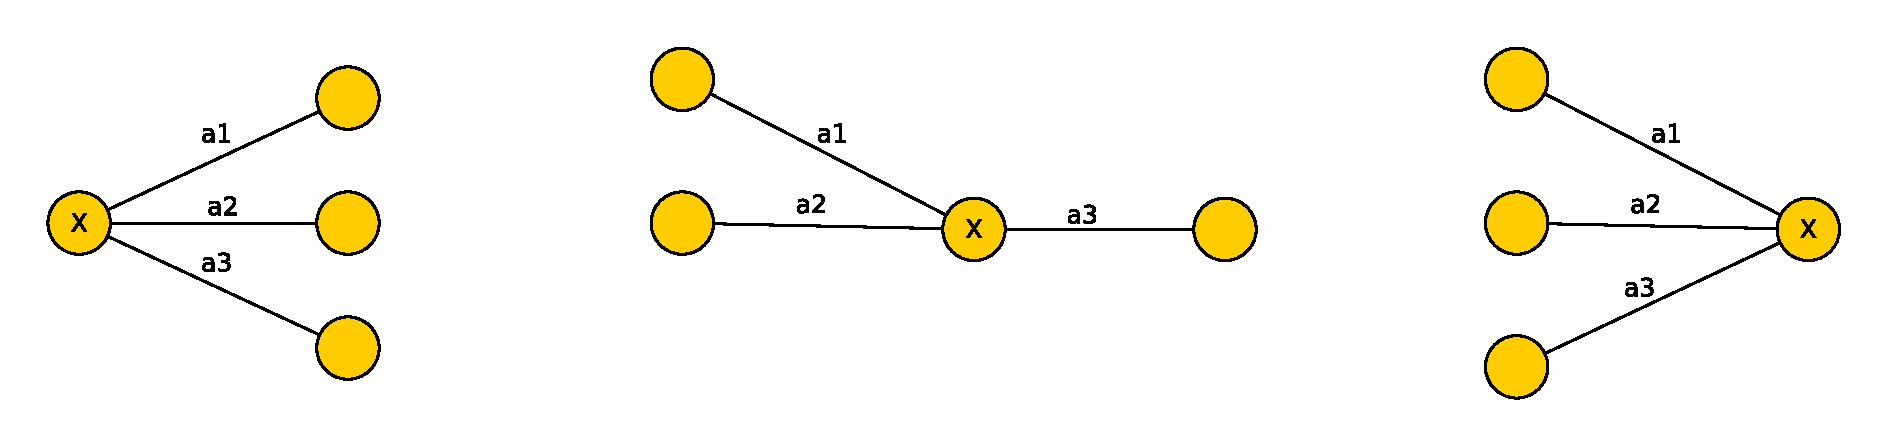
\includegraphics[scale=0.50]{typeSommetsEnCommun.eps}
\caption{De la gauche \`a la droite: sommet $X$ source, sommet $X$ interm\'ediaire, sommet $X$ destination}
\label{typeSommetEnCommun} 
\end{figure}
\end{definition}
Dans la matrice d'adjacence $matE$ de $L(G)$, une case \`a $\mu[i,j] = 1$ d\'esigne deux ar\^etes partageant un sommet dans $G$ alors que la case \`a $\mu[i,j] = 0$ implique que deux ar\^etes n'ont aucuns sommets en commun dans $G$. 
\newline
Par ailleurs, une case \`a $\mu[i,j] = 1$ signifie que sa valeur de corr\'elation  est comprise entre $s$ et $1$ ($s \le \mu_c[i,j] \le 1$) tandis que une case \`a $\mu[i,j] = 0$ implique une valeur de corr\'elation comprise entre $0$ et $s$ ($0 \le \mu_c[i,j] < s$). 
Dans la r\'ealit\'e, nous avons des corr\'elations ($0 \le \mu_c[i,j] < s$)  entre des ar\^etes qui ont un sommet en commun et aussi des corr\'elations  ($s \le \mu_c[i,j] \le 1$) pour des ar\^etes ne partageant aucuns sommets. Ces situations engendrent des {\em erreurs de corr\'elations} dans $matE$.

\begin{definition}
Une {\bf erreur de corr\'elation} est la modification de la valeur d'une case $\mu[i,j]$  de la matrice d'adjacence $matE$ de $L(G)$.
\end{definition}
On distingue quatre cat\'egories d'erreurs de corr\'elation, regroup\'ees dans le tableau \ref{categoriesErreursCorrelation}. Il s'agit des corr\'elations 
\begin{itemize}
\item {\bf vrai positives} : Il s'agit de cases $\mu'[i,j] = 1$ dans $matE'$ n'ayant pas \'et\'e modifi\'ees dans la matrice $matE$.
\item {\bf vrai n\'egatives} :  Il s'agit de cases $\mu'[i,j] = 0$ dans $matE'$ n'ayant pas \'et\'e modifi\'ees dans la matrice $matE$.
\item {\bf faux positives} : Il s'agit de cases $\mu'[i,j] = 0$ dans $matE'$ modifi\'ees dans la matrice $matE$.
\item {\bf faux n\'egatives} : Il s'agit de cases $\mu'[i,j] = 1$ dans $matE'$ modifi\'ees dans la matrice $matE$.
\end{itemize}
% La corr\'elation {\em fausse n\'egative} (l'absence de corr\'elation) est d\'esign\'ee par la valeur $0$ dans la matrice d'adjacence $matE'$ tandis que la corr\'elation {\em fausse positive} (l'existence de corr\'elation) a une valeur $1$ dans cette matrice. (voir tableau \ref{categoriesErreursCorrelation})
  La corr\'elation {\em fausse n\'egative} (l'absence de corr\'elation) est d\'esign\'ee par la valeur $0$ dans la matrice d'adjacence $matE'$ alors que sa case correspondante dans la matrice $matE$ a la valeur $1$. De m\^eme, dans  une corr\'elation {\em fausse positive} (l'existence de corr\'elation), la case  de valeur $1$ dans la matrice $matE'$ est transform\'ee en $0$ dans la matrice $matE$. (voir tableau \ref{categoriesErreursCorrelation}).
\begin{table}[h]
	\centering
	\begin{tabular}{ p{3em} p{3em} p{10em} }
		$L(G)$ & $L(G')$ & $\hspace{1 em}$ corr\'elations \\
		0 & 0 & $\rightarrow$ vrai n\'egative \\
		0 & 1 & $\rightarrow$ fausse positive \\
		1 & 0 & $\rightarrow$ fausse n\'egative \\
		1 & 1 & $\rightarrow$ vrai positive \\
	\end{tabular}
	\caption{ \label{categoriesErreursCorrelation}  Les types d'erreurs dans les matrices d'adjacence de $L(G)$ et $L(G')$}
\end{table}
\newline
% comment departager les erreurs de correlations? p_correl
% quel est la valeur de correlation pour chaque erreur de correlation
La distinction entre ces erreurs est faite par le seuil d'erreur de corr\'elation $p\_correl$.

\begin{definition} {seuil d'erreur de corr\'elation } \newline
Le seuil d'erreur de corr\'elation $p\_correl$ est une valeur de corr\'elation s\'eparant les erreurs de corr\'elations en deux sous-ensembles disjoints. Ce sont l'ensemble des corr\'elations faux n\'egatifs $S_{FN}$ et l'ensemble des corr\'elations faux positives $S_{FP}$. \newline
Si  $p\_correl \le \mu_c[i,j]< s$ $\rightarrow$ on a l'ensemble des corr\'elations fausses positives. \newline
Si $s - p\_correl  \le \mu_c[i,j]< p\_correl$ $\rightarrow$  on a l'ensemble des corr\'elations fausses n\'egatives.
\end{definition}

\begin{figure}[htb!] 
\centering
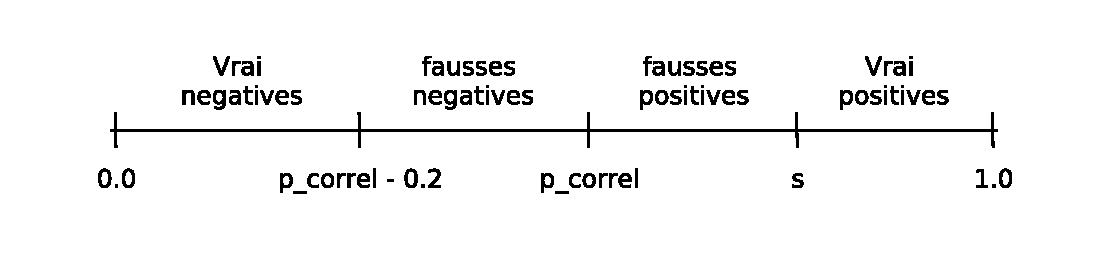
\includegraphics[scale=0.750]{intervallesFauxPositivesNegatives.eps}
\caption{ Correspondance entre valeurs et types de corr\'elations }
\label{intervallesFauxPositivesNegatives} 
\end{figure}

La figure \ref{intervallesFauxPositivesNegatives} r\'esume les valeurs de corr\'elations prises par chaque erreur. Ces valeurs sont regroup\'ees en quatre intervalles :
\begin{itemize}
\item {\em vrai n\'egatives} $\rightarrow$ $int\_vn = [0, s - p\_correl[$
\item {\em fausses n\'egatives} $\rightarrow$ $int\_fn = [s - p\_correl , p\_correl[$
\item {\em fausse positives} $\rightarrow$ $int\_fp = [p\_correl, s[$
\item {\em vrai positives} $\rightarrow$ $int\_vp = [s, 1]$
\end{itemize}

A REVOIR AVEC SERGES
\newline 
Nous affirmons que nous avons que plus corr\'elations {\em fausses positives}  que de corr\'elations fausses n\'egatives ($|S_{FP}| > |S_{FN}|$) quand  $p\_correl \rightarrow s$ alors  que le cardinal des corr\'elations fausses positives $S_{PF}$ est n\'egligeable par rapport \`a celui des  corr\'elations fausses n\'egatives $S_{PN}$ lorsque $p\_correl \rightarrow 0$
Dans le cas o\`u la matrice $matE$ ne contient aucunes erreurs de corr\'elations, alors $p\_correl = s$.

% graphe de correlation
\begin{definition}{ graphe de corr\'elation } \newline
Un graphe de corr\'elation $G'$ est un line-graphe dont on a introduit des erreurs de corr\'elation.
\end{definition}
G\'en\'eralement, le graphe de corr\'elation $G'$ n'est pas  un line-graphe. Toutefois, s'il est un line-graphe alors son graphe racine $L^{-1}(G')$ est diff\'erent du graphe $G$ ($G \neq L^{-1}(G')$).
% methode de correction
\begin{definition}{ m\'ethode de correction } \newline
Un m\'ethode de correction est l'ordre dans lequel on traite des sommets non couverts par aucune clique dans l'algorithme de correction.
\end{definition}

% fonction de cout
\begin{definition}{ fonction de co\^ut d'un sommet} \newline
La fonction de co\^ut d'un sommet est le co\^ut de chaque ar\^ete, ar\^ete ajout\'ee ou supprim\'ee au voisinage du sommet lorsqu'on applique l'algorithme de correction sur ce dernier.
\end{definition}

\subsection{Objectifs}
Le but de cette \'etude est de montrer que nos algorithmes (couverture et correction) proposent
toujours un line-graphe connexe de distance de Hamming minimale 
\`a condition que la matrice du graphe de corr\'elation contienne $k<6$ d'erreurs de corr\'elations
et que les corr\'elations {\bf fausses n\'egatives} repr\'esentent plus de $65\%$ des erreurs de la matrice de corr\'elation.
Ainsi, pour atteindre ce resultat, nous montrerons que la permutation al\'eatoire des sommets \`a corriger est la meilleure m\'ethode de correction et que les valeurs de corr\'elations sont meilleurs pour le calcul du co\^ut des ar\^etes.
Nous pr\'esenterons aussi la relation existance entre la distance line et celle de Hamming afin d'utiliser la distance line comme une m\'etrique dans les cas o\`u il est impossible de calculer la distance de Hamming (cas du graphe iourte).

%##########################################
%#               generation  graphes de correlation				  #
%# 			(protocole de simulation)					  #
%##########################################
\section{G\'en\'eration d'un graphe de corr\'elation}
\label{generationReseauxFlots}
Pour obtenir un graphe de corr\'elation $G'$, nous g\'en\'erons un r\'eseau de flots et nous  lui associons des mesures \'electriques sur chacune des ar\^etes. Ensuite, nous produisons la matrice de  corr\'elation binaire $matE$ li\'ee \`a ce r\'eseau. Enfin nous introduisons $k$ erreurs de corr\'elations dans la matrice $matE$.

\subsection{Construction d'un r\'eseau \'energ\'etique $G$}
Soient $n$ le nombre de sommets et $m$ le nombre d'ar\^etes.
On choisit $\alpha$ le degr\'e moyen de $G$.
\newline
On g\'en\`ere un graphe $G$ de $n$ sommets, de $m$ ar\^etes et dont la probabilit\'e d'existence d'une ar\^ete entre deux sommets est de $\frac{\alpha}{n}$. Si $G$ n'est pas connexe, nous choisissons al\'eatoirement un sommet de chaque composante connexe et nous ajoutons une ar\^ete entre ces sommets. 
\newline
Nous s\'electionnons les sommets de degr\'e minimum comme des sources de notre tri topologique.
Nous effectuons ce tri avec un parcours en largeur {\em Breast First Search (BFS)} dans le graphe $G$.
Chaque sommet $x$ a un ordre topologique $D_x$ et l'ar\^ete $a_{xy}$ devient soit l'arc $a_{xy}$ si $D_x < D_y$ soit l'arc $a_{yx}$ si $D_x > D_y$. 
Le graphe obtenu est alors orient\'e (un {\em DAG} {\em Directed Acyclic Graph} ).
\newline
L'ajout des mesures depend du r\'eseau \'energ\'etique \`a mod\'eliser et des grandeurs physiques \`a observer. 
Dans le cas d'un r\'eseau \'electrique basse tension sinusoidal, nous choisissons l'intensit\'e ($I$), la tension ($U$) et la puissance ($P$) parce que certaines grandeurs physiques n'apportent aucune information (puissance r\'eactive constante ($Q$)) et certains param\`etres du r\'eseau sont inconnus (le facteur de puissance ($cos \phi$)). 
En effet, dans un reseau \'electrique r\'eel, l'intensit\'e varie entre $150A$ et $200A$, la tension entre  $220V$ et $250V$. 
En supposant que la r\'esistance des c\^ables \'electriques est n\'egligeable et que $cos \phi \approx 1$ , la puissance varie de $33000W$ et $62500W$ en s'inspirant de la formule $P = U \times I \times cos \phi$.
\newline
L'attribution des mesures pour chaque grandeur physique se fait \'egalement par parcours en largeur $(BFS)$. 
En effet,  on d\'ebute par les sommets sources et on g\'en\`ere une valeur al\'eatoire comprise dans l'intervalle de la grandeur physique. 
Chaque arc sortant du sommet source re\c coit  un flot \'egal \`a la somme des flots sur les arcs entrants du sommet source multipli\'ee par le facteur $\epsilon$ (d\'esignant les pertes par effets joules) et divis\'ee par le degr\'e sortant de ce sommet si nous avons comme grandeurs les intensit\'es et les puissances.
Dans le cas de grandeurs comme les tensions, le flot de chaque arc sortant est le flot multipli\'e par le facteur $\epsilon$. 
On propage les valeurs de la grandeur physique jusqu'aux sommets puits (les \'equipements consommateurs d'\'energie).
L'application de ces r\`egles de flots permettent de v\'erifier la {\em loi de conversation des noeuds} \cite{loiDeConservation}.

\subsection{Construction de la matrice de corr\'elation}
\'Etant donn\'e que la corr\'elation entre ar\^etes est indiff\'erente de la position des sommets dans celles-ci, la matrice de corr\'elation binaire est la matrice $matE$ d'adjacence du line-graphe $L(G)= (E, A)$. %sous-jacent au graphe non orient\'e de $G$.
\newline
Nous consid\'erons la symm\'etrie sup\'erieure de $matE$ car $G=(V,E)$ est un graphe non orient\'e. 
Toutes les cases $\mu_G[i,j] = 1$ de $matA$ sont num\'erot\'ees par la paire $(i,j)$ et forment les sommets de la matrice $matE$. Lorsque deux ar\^etes ont un sommet commun c'est-\`a-dire $\mu_G[i,j]  = \mu_G[j,k] $ ou $\mu_G[i,j]  = \mu_G[k,j]$ ou $\mu_G[j,i]  = \mu_G[k,j] $ alors la case de $matE$ re\c coit $1$ ($\mu[i',j'] = 1$ avec $i' = (i,j) \in A$ et $j' = (j,k) \in A$).
\newline
La matrice de correction $M$ contient des valeurs de corr\'elation probabilistes. 
Chaque case $\mu_c[i,j]$ de $M$ contient une corr\'elation calcul\'ee selon  le type d'erreur associ\'e \`a celui-ci. 
Pour ce faire, nous consid\'erons deux cas :
\subsubsection{Cas 1 : $matE$ ne contient pas d'erreurs }
Dans ce cas, la variable de seuil de corr\'elation $p\_correl$ est le seuil $s$ ($p\_correl = s$). 
Nous allons g\'en\'erer des corr\'elations {\em vrai positives}  selon la loi exponentielle de param\`etre $\lambda \ge 2$ et des corr\'elations {\em vrai n\'egatives} selon la loi exponentielle de param\`etre $\lambda \ge -2$. Cela donne des distributions repr\'esent\'ees sur la figure \ref{vraiPositivesNegativesAutourDuSeuil}.
\subsubsection{Cas 2 : $matE$ contient d'erreurs }
Nous distinguons les quatres types d'erreurs de corr\'elations. Les corr\'elations {\em vrai positives} et {\em vrai n\'egatives}  suivent  la loi exponentielle de param\`etre $\lambda \ge 2$ et de param\`etre $\lambda \ge -2$ respectivement. 
Les corr\'elations {\em fausses positives et fausses n\'egatives} se localisent autour du seuil $p\_correl$ et  suivent des lois normales. La figure \ref{distributionErreursCorrelations} pr\'esente les courbes des distributions des  diff\'erentes erreurs de corr\'elation.
\begin{figure}[htb!] 
\centering
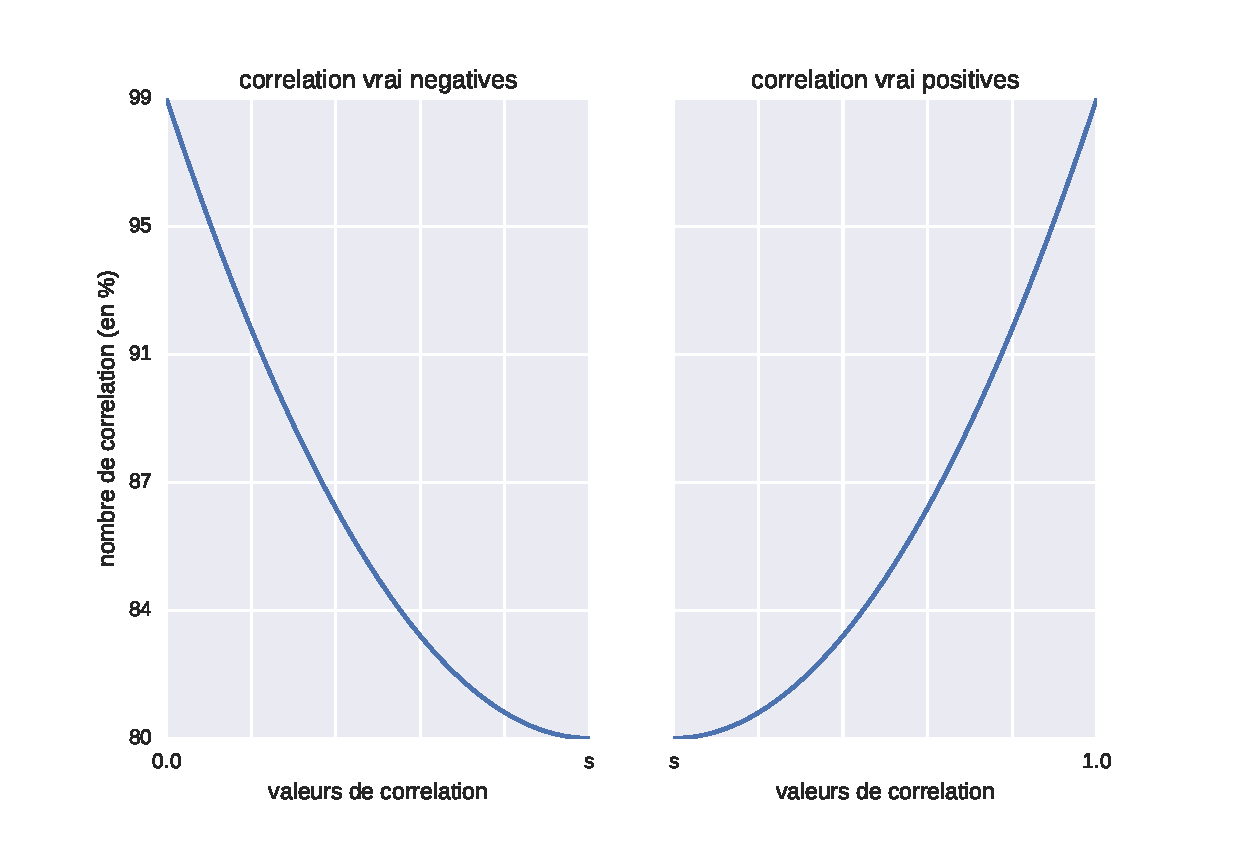
\includegraphics[scale=0.750]{vraiPositivesNegativesAutourDuSeuil.eps}
\caption{\`A gauche : Parabole croissante pour les erreurs {vrai positives} dans l'intervalle  $[s,1]$, \`a droite : Parabole d\'ecroissante pour les erreurs {vrai n\'egatives} dans l'intervalle $[0,s[$. L'ordonn\'e d\'esigne le taux de corr\'elation pour une valeur donn\'ee. }
\label{vraiPositivesNegativesAutourDuSeuil} 
\end{figure}

\begin{figure}[htb!] 
\centering
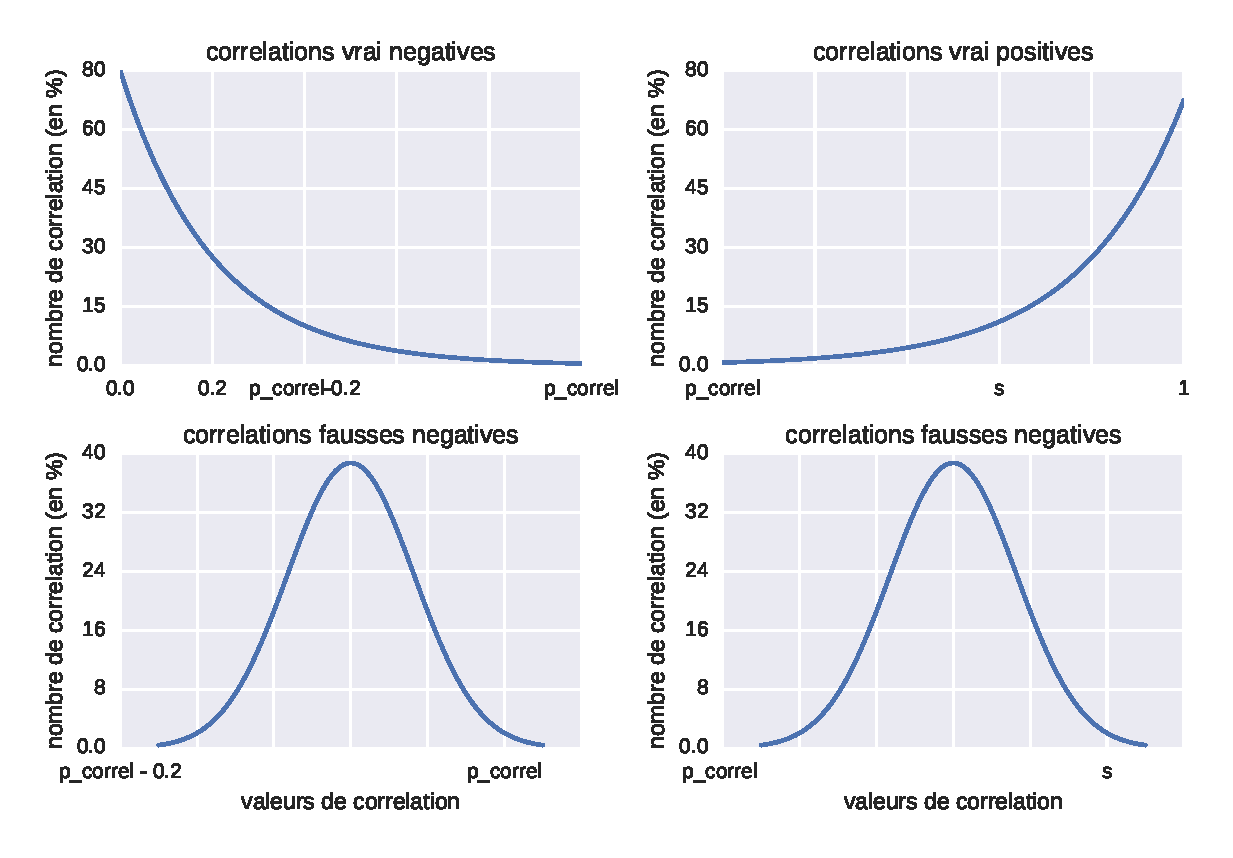
\includegraphics[scale=0.750]{distributionErreursCorrelations.eps}
\caption{En haut : loi exponentielle pour les erreurs   {\em vrai positives et vrai n\'egatives}, en bas : loi uniforme pour les erreurs   {\em fausses positives et fausses n\'egatives} }
\label{distributionErreursCorrelations} 
\end{figure}

 
L'utilisation de lois de probabilit\'e a pour but de montrer l'impact du seuil $p\_correl$ sur la line-couverture et aussi de calculer les co\^uts de correction des sommets n'appartenant \`a aucune clique.

%##########################################
%#               correction graphes de correlation avec erreurs          #
%##########################################
\section{Correction d'un graphe de corr\'elation}
L'initialisation de certains param\`etres est la phase primordiale dans nos algorithmes pour obtenir un line-graphe. Les valeurs de ces param\`etres sont choisies apr\`es l'exp\'erimentation sur des r\'eseaux g\'en\'er\'es, d\'ecrits dans la section \ref{generationReseauxFlots}.

\subsection{Protocole d'exp\'erimentation}
La r\'ealisation de notre \'etude passe par la g\'en\'eration de $500$ graphes de flots $G$ de $30$ sommets ayant un degr\'e maximal moyen $\Delta(G) = 5$ qui simulent le fonctionnement d'un r\'eseau \'electrique. Nous en d\'eduisons \'egalement $500$ line-graphes de $150$ sommets et $470$ ar\^etes, en moyenne. \newline
Nous introduisons trois param\`etres $k, p\_correl, prob$:
\begin{enumerate}
\item $k$ d\'esigne le nombre de corr\'elations erron\'ees \`a ajouter dans la matrice $matE$. Dans notre \'etude, $k \in [1,9]$.
\item $p\_correl$ d\'esigne la probabilit\'e d'ajouter des erreurs de corr\'elations, soit corr\'elation {\em fausses positives} (ajout d'ar\^etes) soit corr\'elation {\em fausses n\'egatives} (suppression d'ar\^etes) soit les deux. Cette variable $p\_correl \in [0,1]$ varie par pas de $0.1$. Ainsi,
	\begin{itemize}
	\item si $p\_correl=0$ $\rightarrow$ la matrice $matE'$ ne contient que des  corr\'elations {\em fausses positives} car on supprime uniquement des ar\^etes dans le line-graphe de matrice d'adjacence $matE$.
	\item si $p\_correl=0.5$ $\rightarrow$ le nombre de corr\'elations {\em fausses n\'egatives} et  {\em fausses positives} est approximativement identique  dans la matrice $matE'$ car on ajoute et supprime \'equiprobablement des ar\^etes dans la matrice $matE$.
	\item si $p\_correl=1.0$ $\rightarrow$ la matrice $matE'$ ne contient que des corr\'elations {\em fausses n\'egatives} car on ajoute des ar\^etes dans le line-graphe de matrice $matE$.
	\end{itemize}
\item $prob$ d\'esigne la probabilit\'e associ\'ee \`a une corr\'elation selon le type d'erreurs rencontr\'e dans $matE'$. En un mot, $prob$ est la valeur de corr\'elation entre ar\^etes.
Ce param\`etre est important car les valeurs de corr\'elations calcul\'ees  ne sont pas binaires mais dependent d'une loi de probabilit\'e. Nous en reparlerons \'egalement dans la section \ref{fonctionDeCout}.
\end{enumerate}
Pour ajouter des erreurs de corr\'elation \`a la matrice $matE$ correcte, on tire al\'eatoirement $k$ cases non encore modifi\'ees. Nous mettons chaque case et sa case sym\'etrique \`a $1$ si la probabilit\'e de la case est inf\'erieure ou \'egale \`a $p\_correl$. Si cette case est d\'ej\`a \`a $1$, on choisit une autre case. Selon le type d'erreurs de chaque case (vrai n\'egatives, vrai positives), on lui attribue une valeur de corr\'elation selon les distributions pr\'ed\'efinies.
\newline

Consid\'erons le graphe $G_k$ de matrice d'adjacence $matE_k$ dans laquelle on ajoute $k \in [1,9]$ erreurs de corr\'elation selon $p\_correl=0.5$, la probabilit\'e d'ajouter autant d'erreurs {\em fausses n\'egatives } que d'erreurs {\em fausses positives}. 
\`A la fin de l'ex\'ecution de l'algorithme de couverture, s'il existe des sommets de $G_k$ non couverts par {\em une ou deux cliques}, on les ajoute \`a l'ensemble des sommets \`a corriger $sommets\_1$ et nous appliquons l'algorithme  de correction sur chaque sommet de $sommets\_1$ selon les m\'ethodes suivantes:
\begin{itemize}
\item m\'ethode 1 : degr\'e minimum avec remise.\newline
Elle consiste \`a s\'electionner le sommet de degr\'e minimum dans l'ensemble $sommets\_1$, \`a appliquer l'algorithme de correction afin de modifier $matE_k$ et enfin  d'ex\'ecuter \`a nouveau les deux algorithmes sur la matrice $matE_k$ modifi\'ee.
\item m\'ethode 2 : co\^ut minimum avec remise. \newline
Elle consiste \`a s\'electionner le sommet de co\^ut minimum dans l'ensemble $sommets\_1$, \`a appliquer l'algorithme de correction pour modifier $matE_k$ et enfin \`a re-ex\'ecuter les deux algorithmes sur la matrice $matE_k$ modifi\'ee.
\item m\'ethode 3 : co\^ut minimum avec permutation des sommets de $sommets\_1$. \newline
Elle consiste \`a choisir une permutation dont les sommets sont class\'es par ordre croissant de leur co\^ut  de modification de la matrice $matE_k$ et \`a appliquer l'algorithme de correction sur cette permutation.
\item m\'ethode 4 :  degr\'e minimum avec  permutation des sommets de $sommets\_1$. \newline
Elle consiste \`a choisir une permutation dont les sommets sont class\'es par ordre croissant de leur degr\'e et \`a appliquer l'algorithme de correction sur cette permutation.
\item m\'ethode 5 : permutation al\'eatoire des sommets de $sommets\_1$. \newline
Elle consiste \`a choisir al\'eatoirement $N$ permutations puis \`a appliquer l'algorithme de correction et \`a s\'electionner la permutation ayant un co\^ut et une distance de Hamming minimum.
\end{itemize}

% calcul de moy_dl et moy_dh
Consid\'erons 
  $\alpha \in [1, 5]$ le nombre de fois qu'on applique $k$ erreurs dans la matrice $matE$ du line-graphe $LG$,  
 $G_{k, \alpha}$ le graphe de matrice d'adjacence $matE_{k, \alpha}$ dont on a modifi\'e $k$ corr\'elations $\alpha$ fois et 
 $LG_{k, \alpha}$  le line-graphe de matrice d'adjacence $matE_{k, \alpha}$ fourni par les algorithmes de couverture et de correction \`a partir du graphe $G_{k, \alpha}$.
\newline
En comparant
\begin{enumerate}
\item  $LG$ et $LG_{k, \alpha}$, on obtient la distance de Hamming not\'ee $DH_{k,\alpha}$.
\item $G_{k,\alpha}$ et $LG_{k,\alpha}$, on obtient la distance line not\'ee $DL_{k,\alpha}$.
\end{enumerate}
On d\'efinit par les variables $moy\_DH$ et $moy\_DL$, les moyennes respectives des distances de Hamming (not\'ee $DH_{k,\alpha}$) et des distances line (not\'ee $DL_{k,\alpha}$) pour une valeur donn\'ee de $k$ et pour tout $\alpha \in [1, 5]$.
\begin{equation}
moy\_DH_k = \sum_{\alpha = 1}^{5} DH_{k, \alpha} \hspace{2 em}
moy\_DL_k = \sum_{\alpha = 1}^{5} DL_{k, \alpha}
\end{equation}

Le protocole d'exp\'erimentation est r\'esum\'e dans la figure \ref{recap_protocole_etude}. Le r\'eseau de flots $G$ g\'en\'er\'e est transform\'e en un line-graphe $LG$, puis $k$ erreurs de corr\'elations  sont ajout\'ees $\alpha$ fois dans $LG$ pour obtenir $G_{k,\alpha}$. Nous appliquons les algorithmes (couverture et correction) pour d\'eterminer la line-couverture (ou la plus proche possible) du graphe $G_{k,\alpha}$ car ce graphe n'est pas n\'ecessairement un line-graphe. Cette line-couverture forme un line-graphe $LG_{k, \alpha}$ proche ou identique au line-graphe $LG$. Le line-graphe $LG_{k, \alpha}$ est utilis\'e pour calculer les distances line ($DL_{k, \alpha}$) et de Hamming ($DH_{k, \alpha}$).
Les valeurs moyennes ($moy\_DL$, $moy\_DH$) des distances line et de Hamming sont calcul\'ees pour chaque erreur $k$ et leurs distributions sont pr\'esent\'ees dans la section suivante afin de montrer les performances des algorithmes en pr\'esence d'erreurs de corr\'elations de diff\'erentes lois de probabilit\'es.
\begin{figure}[htb!] 
\centering
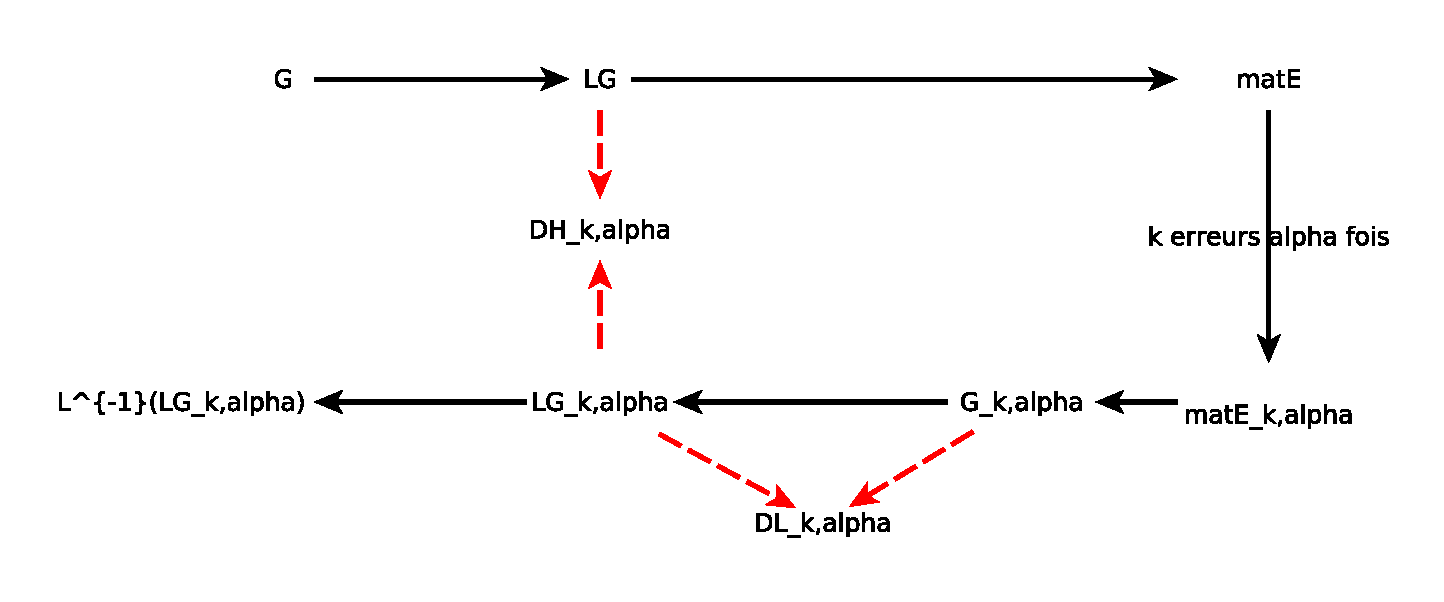
\includegraphics[scale=0.70]{recapProtocoleEtude.eps}
\caption{ Diff\'erentes \'etapes du processus d'exp\'erimentation de nos algorithmes (fl\`eches en noir), calcul de distances entre \'etapes (fl\`eches pointill\'ees en rouge).}
\label{recap_protocole_etude} 
\end{figure}
%---- decription protocole d'etude --> fin
\subsection{Analyses et interpr\'etations}
Les valeurs de corr\'elations sont d\'efinies par les lois uniformes (erreurs vrai positives et vrai n\'egatives) et exponentielles (erreurs fausses positives et fausses n\'egatives) comme illustr\'e par la figure \ref{distributionErreursCorrelations} pour une probabilit\'e d'ajout des erreurs $p\_correl = 0.5$. 
Cette valeur $p\_correl$  signifie qu'il y a autant d'erreurs fausses positives que d'erreurs fausses n\'egatives dans la matrice de corr\'elation du graphe $G_{k}$. 
Ces lois de distribution respectent l'hypoth\`ese de corr\'elations des arcs. Cette hypoth\`ese affirme que deux arcs correl\'es ont leur valeur de correction qui tende vers $1$ alors qu'une valeur proche de $0$ d\'esigne des arcs non correl\'es. 
\newline
% interpretation d'une distribution  DH et DL pour une methode
% presentation des differentes methodes et comparaison
% comparaison entre differentes p
% impact de la fonction de cout
Nous d\'ecrirons d'abord les distributions des distances line et de Hamming moyenn\'ees ($moy\_DL$ ou $moy\_DH$) pour une m\'ethode de correction (al\'eatoire). Ensuite nous comparons les cinq m\'ethodes de correction en nous basant sur les distances de Hamming moyenn\'ees. 
Enfin nous expliquons le choix de la m\'ethode de {\em permutation al\'eatoire} et montrons que les algorithmes (couverture et correction) proposent de meilleurs r\'esultats lorsque la matrice de corr\'elation poss\`ede plus de corr\'elations {\em faux n\'egatives} que de corr\'elations {\em faux positives} et aussi peu d'erreurs de corr\'elations ($k < 6$). 
\newline
Nous pr\'esentons \'egalement l'impact de la fonction de co\^ut dans les distributions  de distances de Hamming et 
la relation existante entre la distance line et la distance de Hamming.
\subsubsection{Distribution de la m\'ethode de permutation al\'eatoire}
% description distribution methode aleatoire
% expliquer les distributions moy_dh et moy_dl  et les courbes de ces distributions pour une methode de correction
% interpretation selon loi uniforme  pour p = 0.5
% k = [0,5] : une figure
% k = [6,9] : une autre figure
% k = [10,50] : une autre figure
% cas particulier pour la loi de poisson

%\begin{figure}[htb!] 
%\centering
%%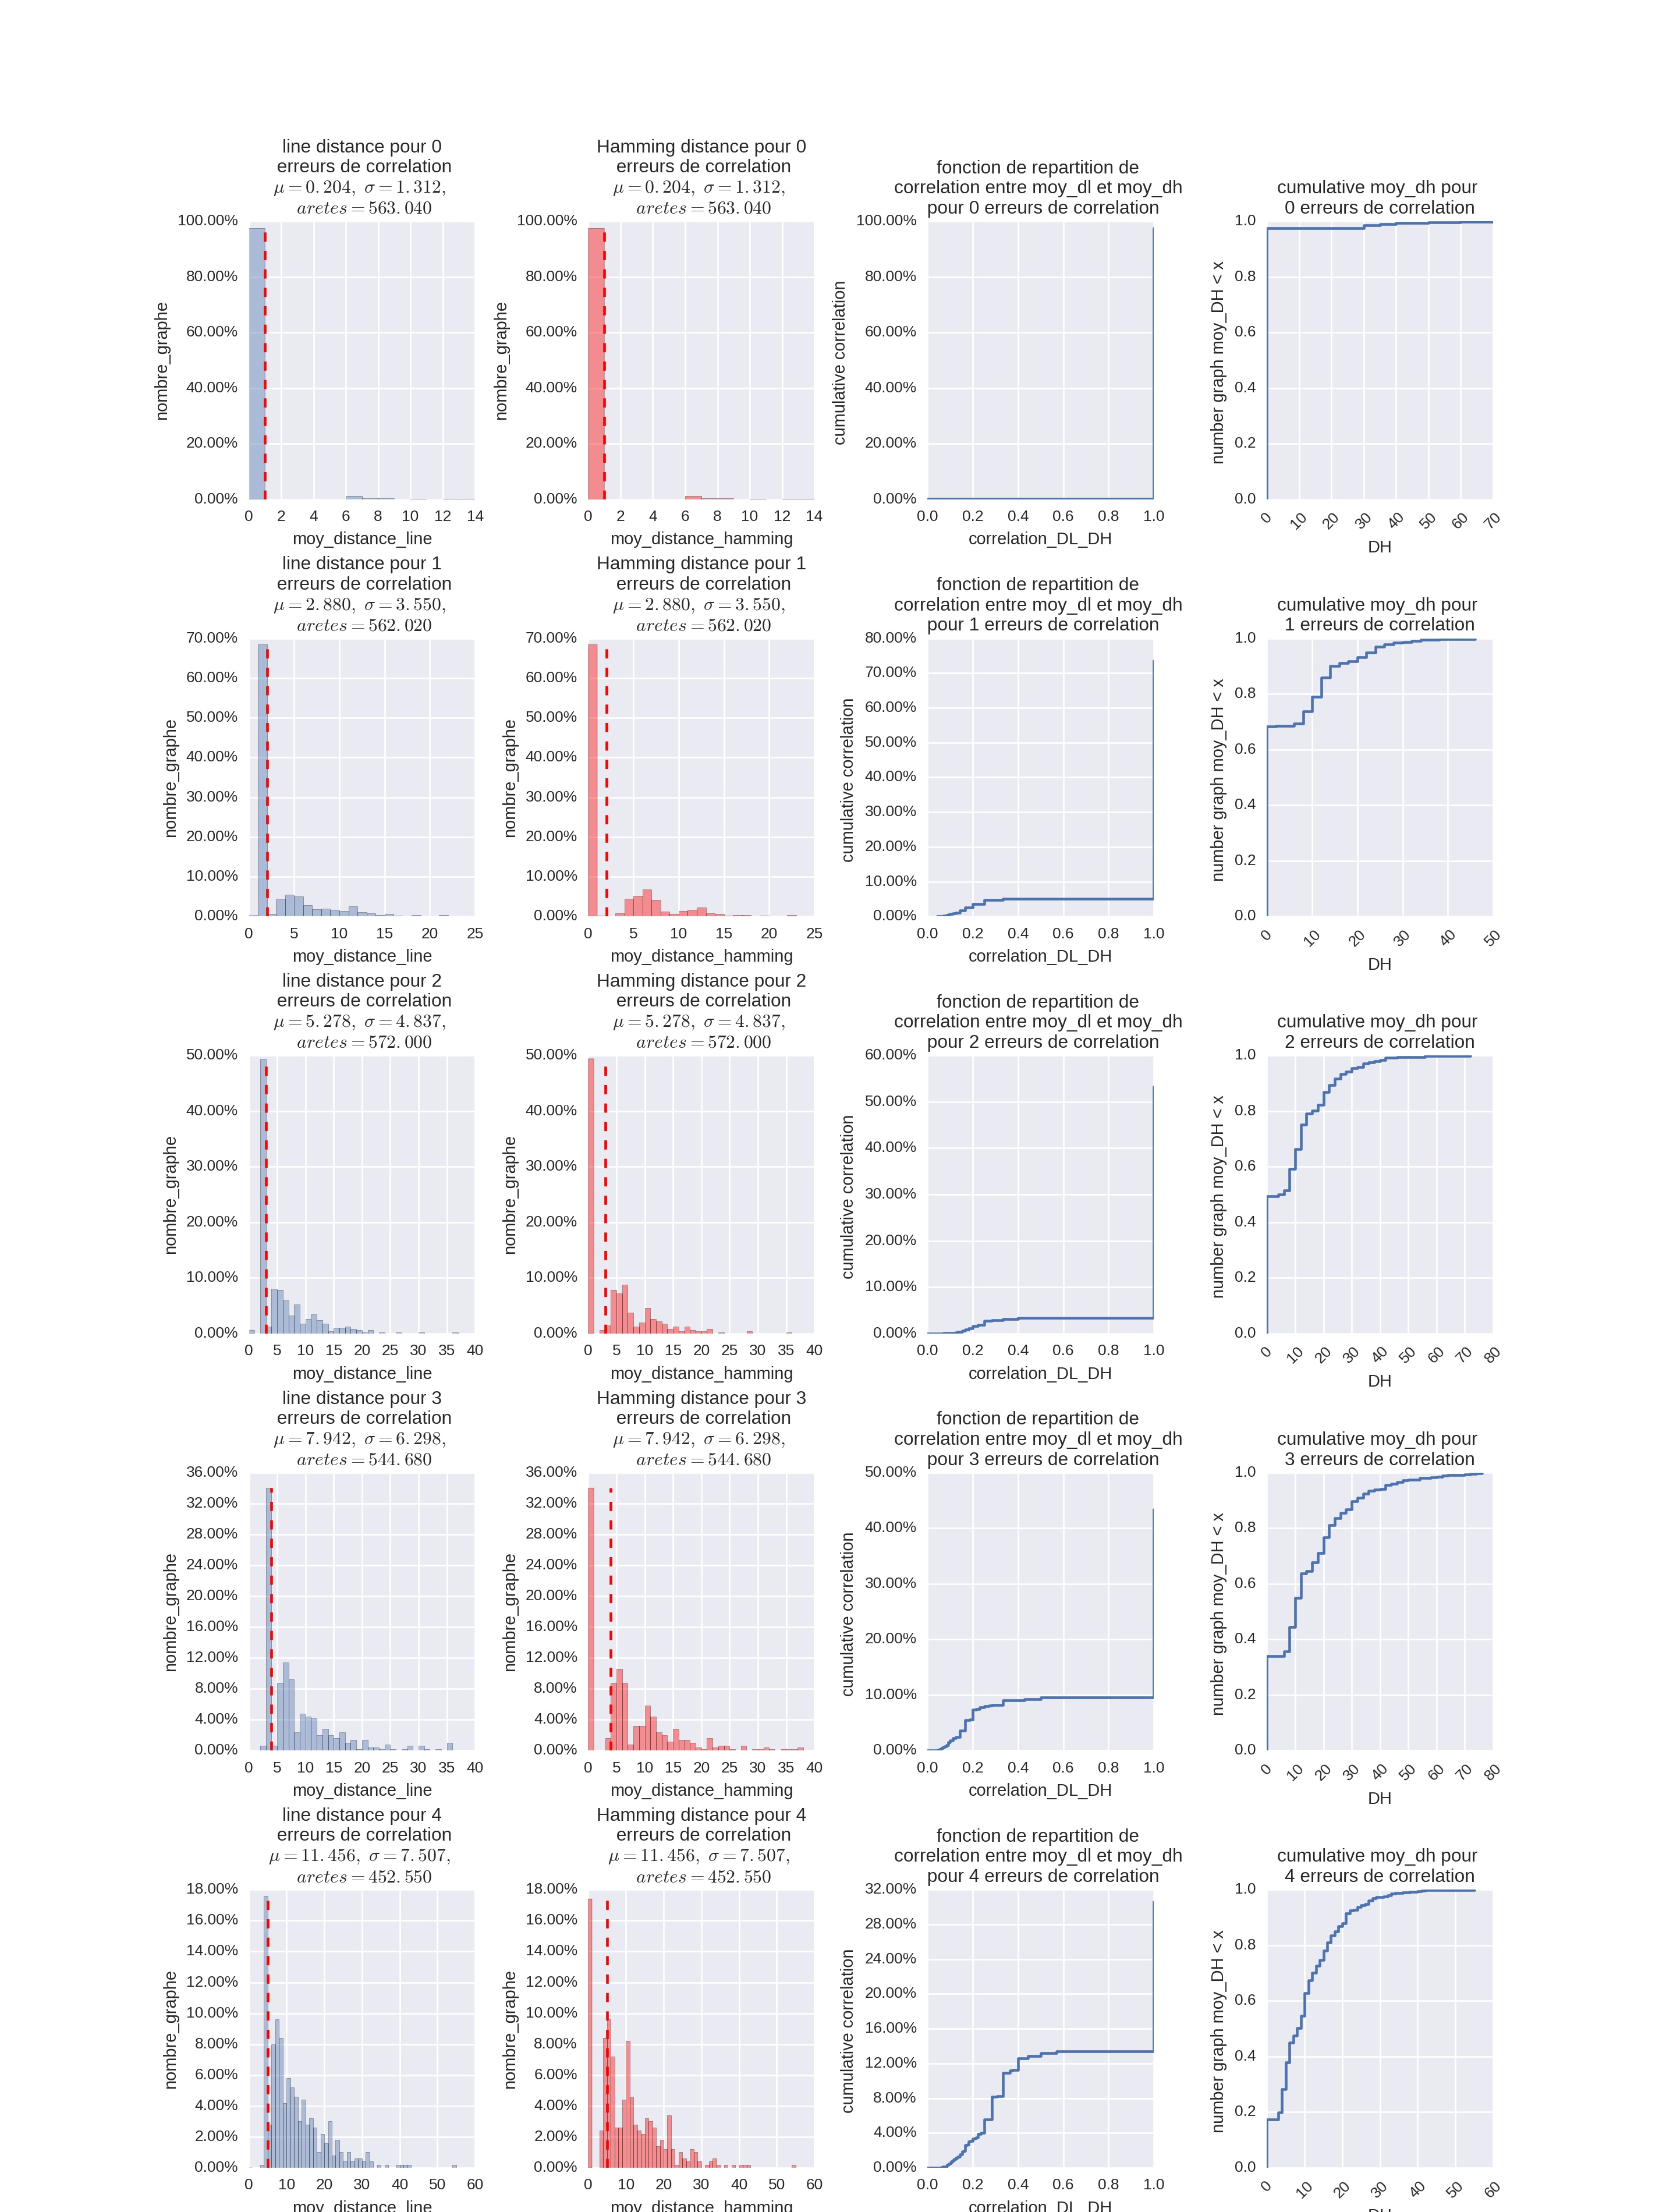
\includegraphics[scale=0.150]{permut_distanceMoyenDLDH_k_0_4_aleatoire_p_05.jpeg}
%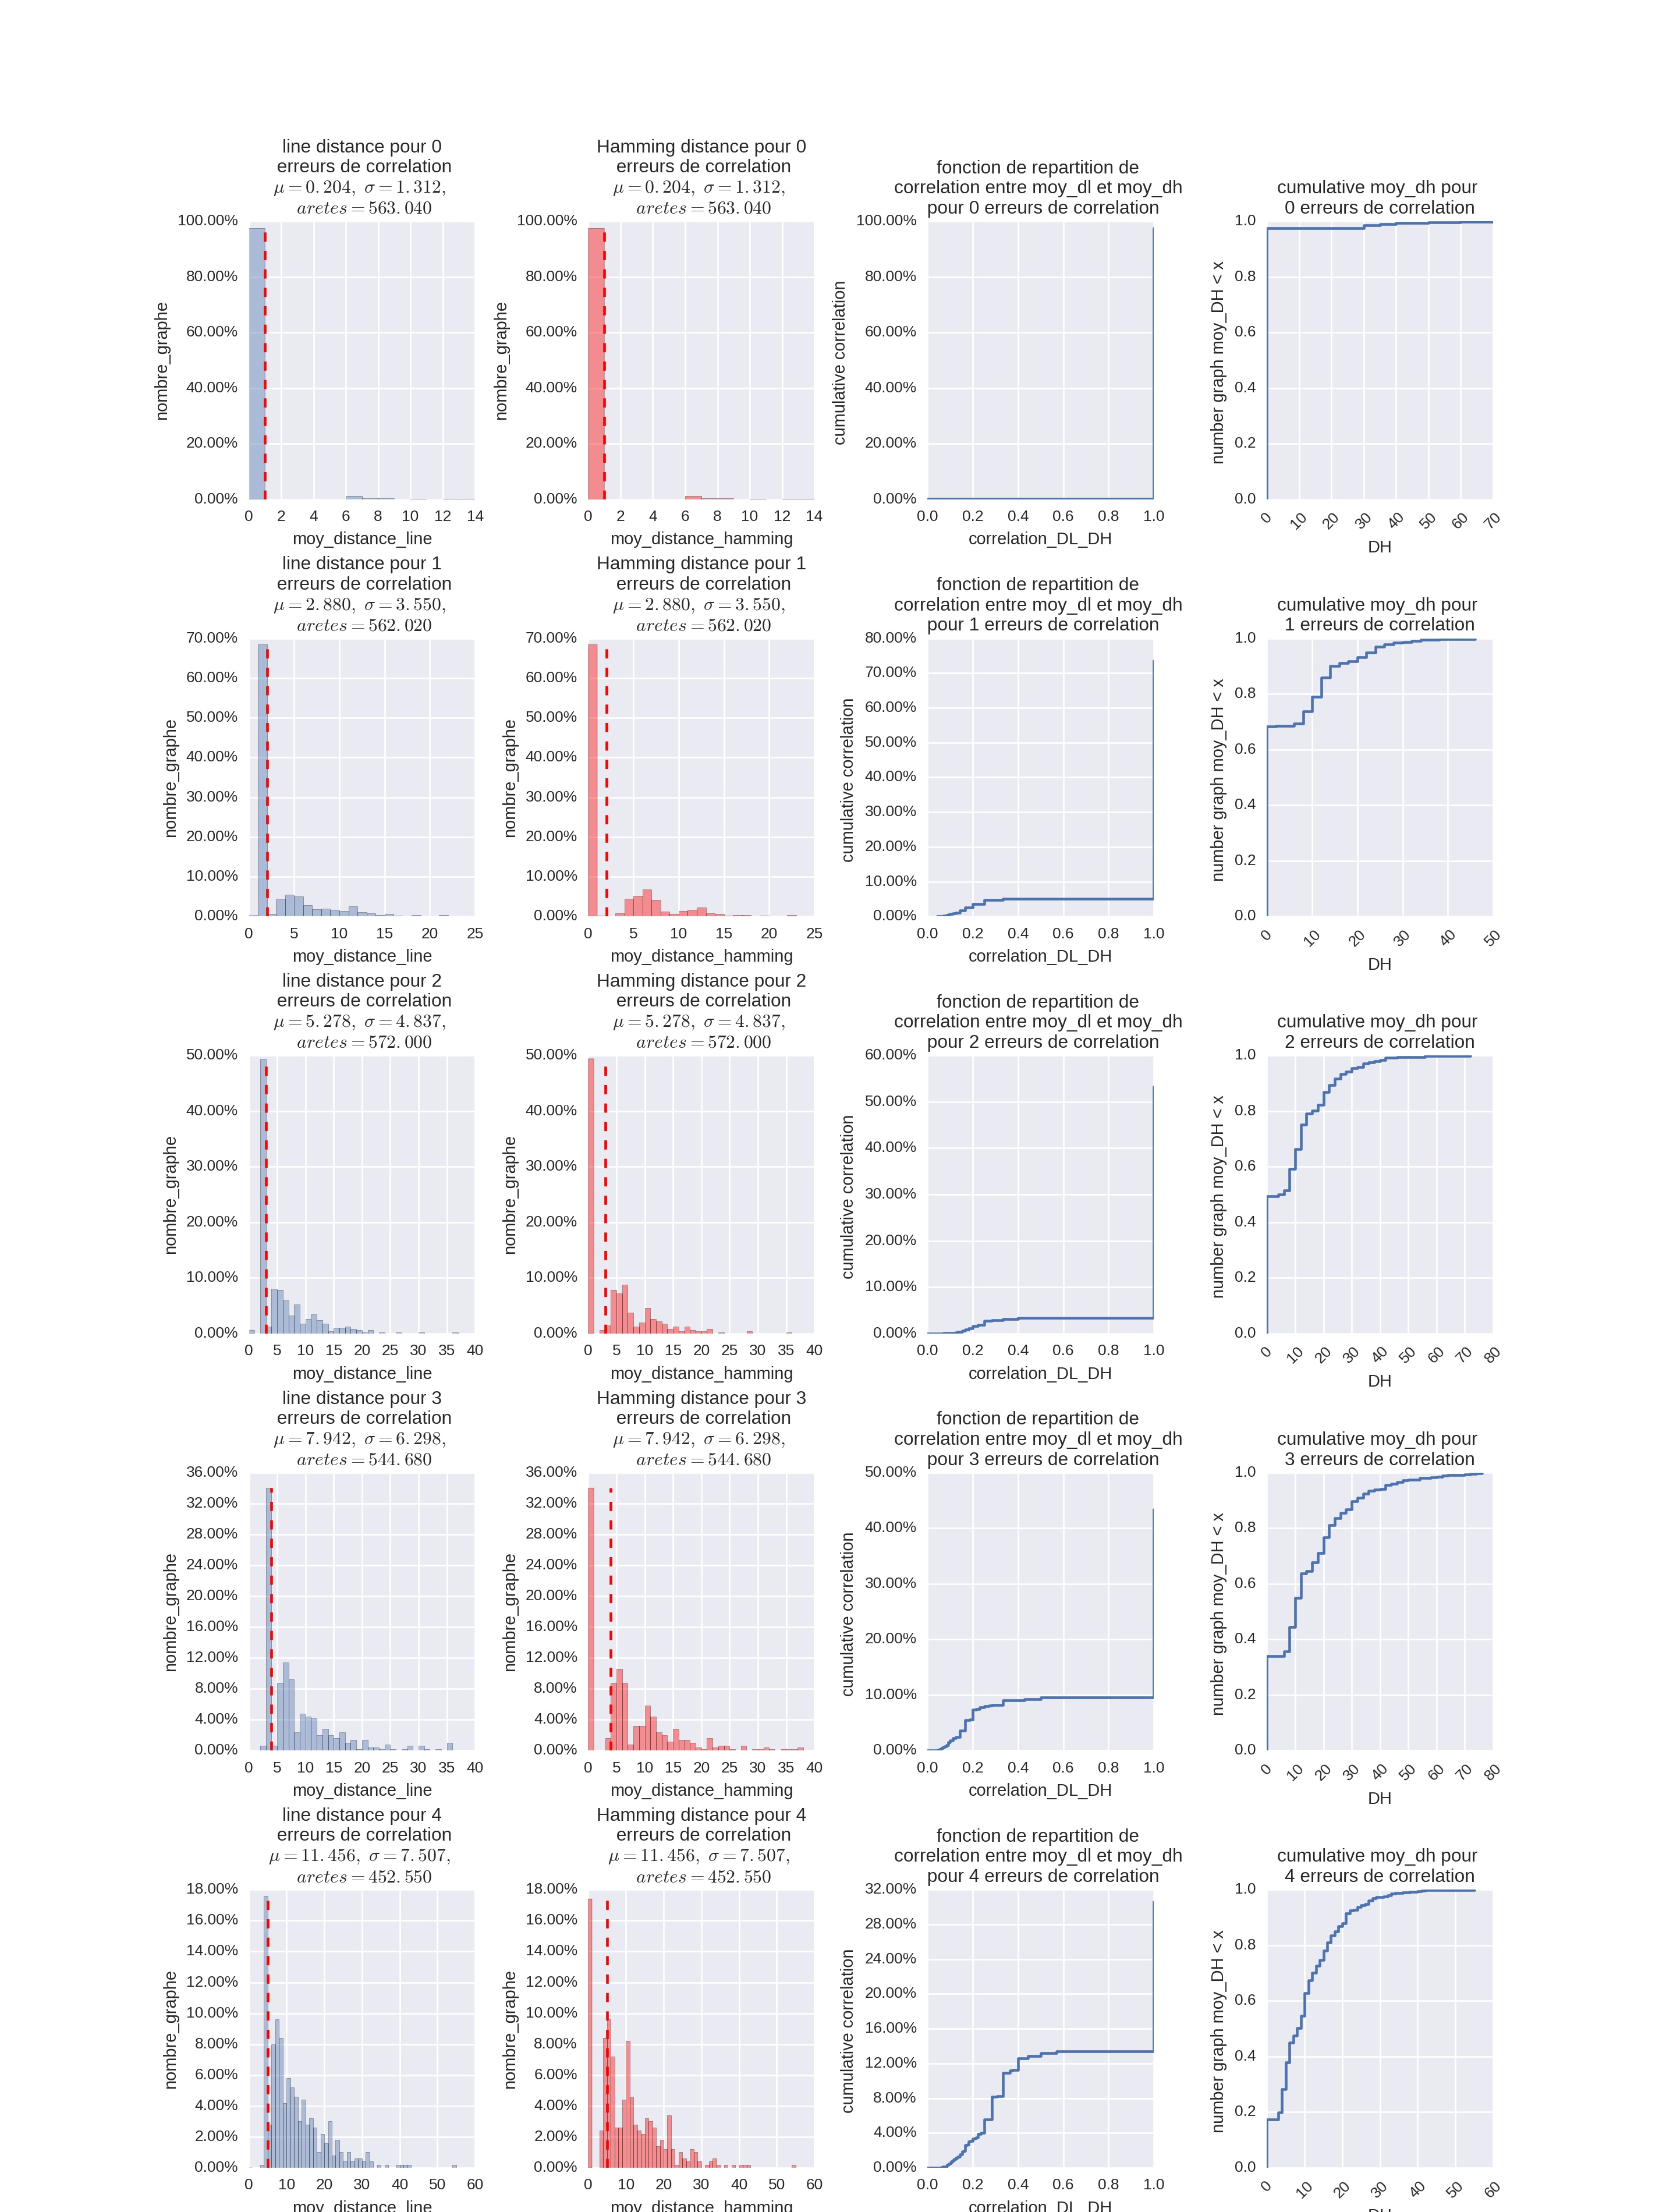
\includegraphics[width=550pt, height=600pt]{permut_distanceMoyenDLDH_k_0_4_aleatoire_p_05.jpeg}
%\caption{ M\'ethode de permutation al\'eatoire avec une fonction de correction \`a co\^ut unitaire : distribution des distances line $moy\_DL$ et de Hamming $moy\_DH$ pour $k \in [0,  5]$ corr\'elations alter\'ees}
%\label{permut_distanceMoyenDLDH_k_0_5_aleatoire_p_05} 
%\end{figure}

\begin{figure}[htb!] 
\centering
\includegraphics[width=500pt,height=160pt]{simulation_distanceMoyenDLDH_k_0_aleatoire_p_05.jpeg}
\caption{ M\'ethode de permutation al\'eatoire avec une fonction de correction \`a co\^ut unitaire : distribution des distances line $moy\_DL$ et de Hamming $moy\_DH$ pour $k =0 $ corr\'elation alter\'e}
\label{permut_distanceMoyenDLDH_k_0_aleatoire_p_05} 
\end{figure}

\begin{figure}[htb!] 
\centering
\includegraphics[width=550pt,height=600pt]{permut_distanceMoyenDLDH_k_1_2_5_9_aleatoire_p_05.jpeg}
\caption{ M\'ethode de permutation al\'eatoire avec une fonction de correction \`a co\^ut unitaire : distribution des distances line $moy\_DL$ et de Hamming $moy\_DH$ pour $k \in [1,2,5, 9]$ corr\'elations alter\'ees}
\label{permut_distanceMoyenDLDH_k_1_2_5_9_aleatoire_p_05} 
\end{figure}

%\begin{figure}[htb!] 
%\centering
%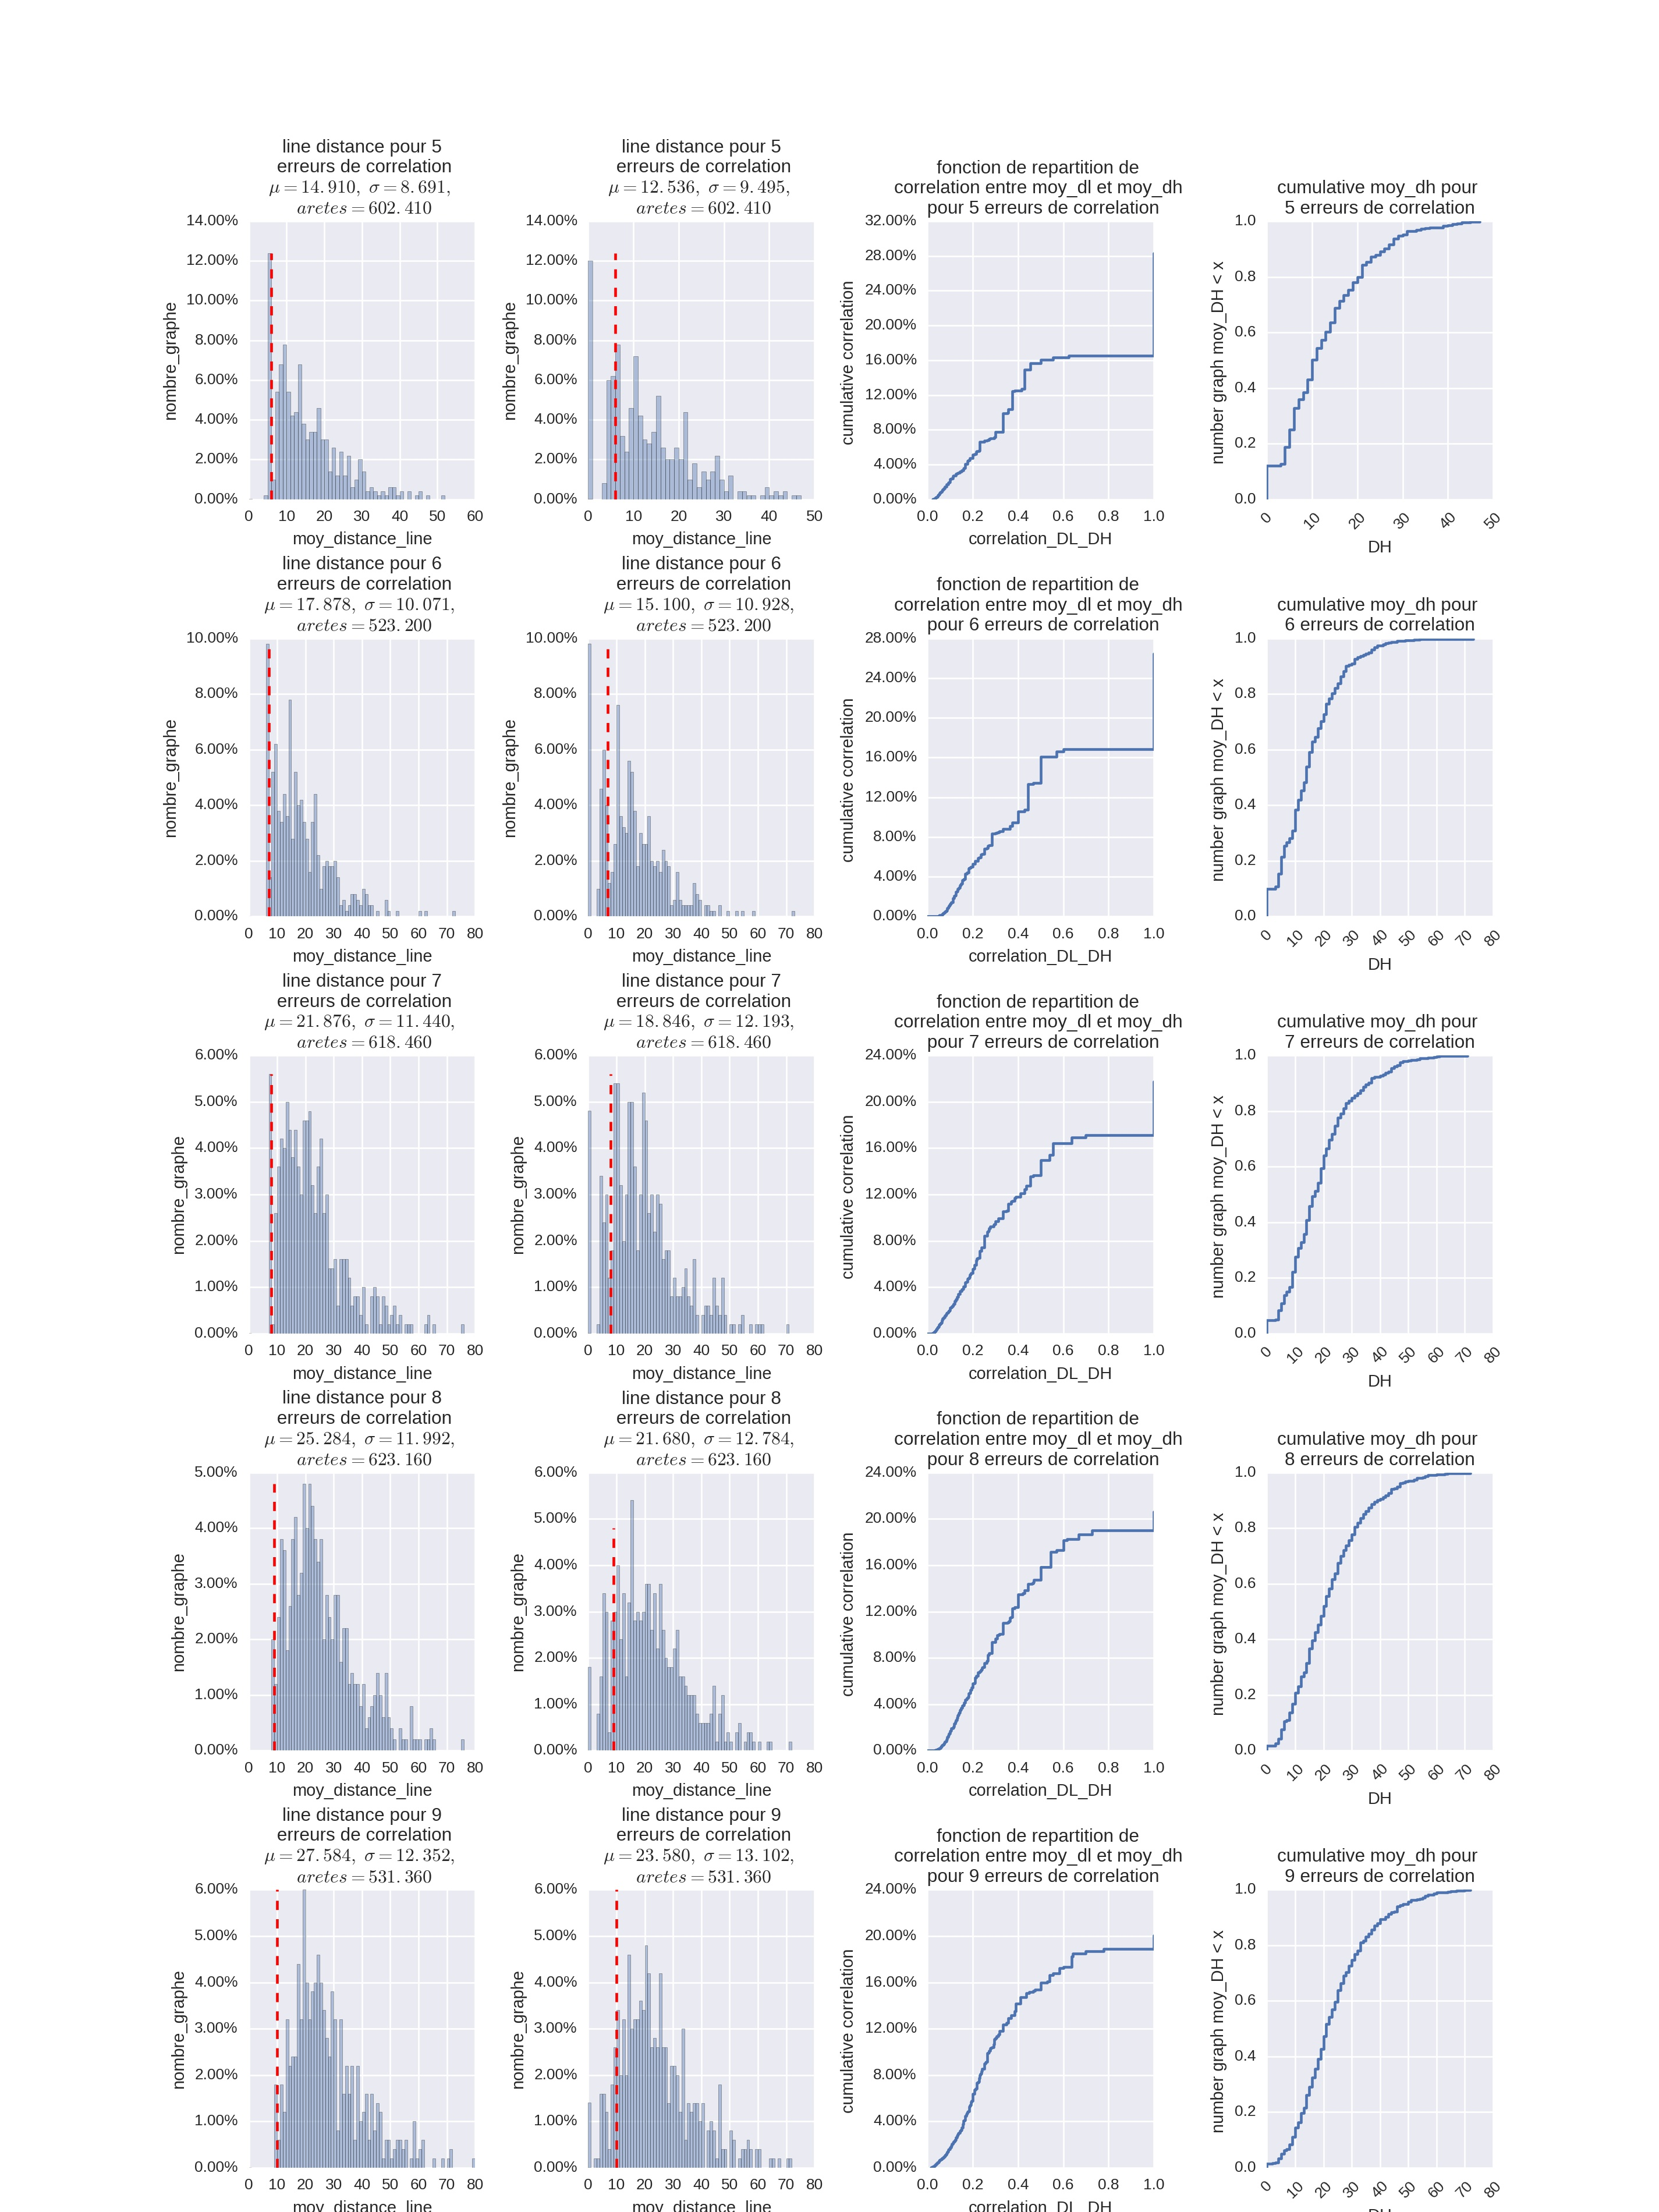
\includegraphics[width=550pt,height=600pt]{permut_distanceMoyenDLDH_k_5_9_aleatoire_p_05.jpeg}
%\caption{ M\'ethode de permutation al\'eatoire avec une fonction de correction \`a co\^ut unitaire : distribution des distances line $moy\_DL$ et de Hamming $moy\_DH$ pour $k \in [6,  9]$ corr\'elations alter\'ees}
%\label{permut_distanceMoyenDLDH_k_5_9_aleatoire_p_05} 
%\end{figure}

La figure \ref{permut_distanceMoyenDLDH_k_1_2_5_9_aleatoire_p_05} repr\'esente les distributions des distances line, de Hamming, des fonctions de r\'epartition de la corr\'elation entre les distances line et  de Hamming pour $k \in [1,2,5,9]$ erreurs. 
\newline
Pour $k=0$ erreur (figure \ref{permut_distanceMoyenDLDH_k_0_aleatoire_p_05}), nous avons un batonnet sur les histogrammes de distances line et de Hamming. Ce batonnet est le pourcentage d'ar\^etes identiques entre les graphes $G_k$ et $LG_k$ (distance line) et aussi entre les graphes  $LG$ et $LG_k$ (distance de Hamming). Nous remarquons que le pourcentage d'ar\^etes identiques est de $100\%$ et cela signifie que les graphes $LG_k$ et $LG$ sont isomorphes en ar\^etes c'est-\`a-dire que les ar\^etes des graphes $LG_k$ et $LG$ sont identiques. Ce qui est normal parce que nous n'avons ajout\'e aucune erreur dans le line-graphe $LG$. 
Par ailleurs, nous avons deux fonctions de r\'epartition. La premi\`ere fonction $y_{correlDLDH}^{0}$ calcule la corr\'elation entre les distances line et de Hamming. Elle est d\'efinie par l'\'equation \ref{eqCorrelMoyDLDH} et se localise dans la troisi\`eme colonne de la figure \ref{permut_distanceMoyenDLDH_k_1_2_5_9_aleatoire_p_05}. La deuxi\`eme fonction $y_{cumulDH}^{0}$, d\'efinie par l'\'equation \ref{eqCumulMoyDH}, calcule les corr\'elations cumul\'ees des distances de Hamming et occupe la quatri\`eme colonne de la figure \ref{permut_distanceMoyenDLDH_k_1_2_5_9_aleatoire_p_05}.
\begin{equation}
\label{eqCorrelMoyDLDH}
y_{correlDLDH}^{0} = \left\{
	\begin{aligned}
	0 \hspace{1 em} si \hspace{1 em} x < 1 \\
	100  \hspace{1 em}  si  \hspace{1 em}  x = 1
	\end{aligned}
	\right.
\end{equation}
\begin{equation}
\label{eqCumulMoyDH}
y_{cumulDH}^{0} = 1  \hspace{1 em}  si  \hspace{1 em}   x \in [0,1]
\end{equation}
La variable $x$ est la corr\'elation entre la distance line et la distance de Hamming.
En effet,  $x = 1$ implique que $DL = k$ et $DH = 0$ tandis que  $x = 0$ implique que $DL = k$ et $DH = k$.
L'\'equation  \ref{eqCorrelMoyDLDH} s'interpr\`ete comme suit : $y_{correlDLDH}^{0} = 100\%$ des line-graphes ont leur distance line et de Hamming correl\'ees ($x = 1$).
Le cas de $k=0$ erreur servira de r\'ef\'erence pour la meilleure performance de nos algorithmes.
\newline
%-- pour k \in [1,2]
Pour $k \in [1,2]$, dans la premi\`ere et seconde colonne, le batonnet de pic maximal est \`a gauche de la droite $y = k$ (droite en rouge) de chaque histogramme et  son pourcentage est sup\'erieur \`a $50 \%$. Les autres batonnets sont regroup\'es \`a droite de $y = k$ et le pic maximal du pourcentage de ces batonnets est inf\'erieur \`a $10\%$. La droite $y = k$ d\'esigne le nombre d'erreurs ajout\'ees dans le graphe de corr\'elation $G_k$.
Dans la seconde colonne, le pic correspond \`a $moy\_DH = 0$ ar\^ete indiquant qu'il n'y a aucune diff\'erence d'ar\^etes entre les  graphes $G_k$ et $LG_k$. Dans la premi\`ere colonne, le pic correspond \`a $k$ erreurs et son pourcentage est identique \`a celui de $k=0$ dans la seconde colonne. Cela signifie que les $k$ erreurs ajout\'ees dans $G_k$ ont \'et\'e supprim\'ees. Ainsi, nous retrouvons le line-graphe initial dans un cas sur deux lorsque nous ajoutons $k \le 2$ erreurs.
% par ailleurs comment se comporte les algos lorsque les k erreurs ne sont pas corrigees
Cependant, on observe que les distances line et de Hamming  ont approximativement les m\^emes valeurs lorsque les $k$ erreurs n'ont pas \'et\'e corrig\'ees. 
En effet, pour $x > 0.3$, $y_{correlDLDH}^{k} > 60\%$ et  pour $x \le 0.3$, $y_{correlDLDH}^{k} < 5\%$ (voir troisi\`eme colonne figure \ref{permut_distanceMoyenDLDH_k_1_2_5_9_aleatoire_p_05}). Or $y_{correlDLDH}^{k} \rightarrow 0\%$ signifie que $DL$ est \'egale \`a $k$ ($DL = k$) et $DH$ tend vers $k$ ($DH \rightarrow k$). Donc $y_{correlDLDH}^{k} < 5\%$ implique que $DL = k$ et $DH \approx k$.
Ainsi, les distances line et de hamming sont corr\'el\'ees dans $5\%$ des line-graphes et le line-graphe $LG_k$, d\'ecouvert par les algorithmes, devient  au line-graphe initial $LG$ si nous retirons/ajout\'ons les $DL$ ar\^etes du graphe $LG_k$.
\newline
%-- pour k \in [5,9] 
Pour $k  = 5$ erreurs,  le pic de chaque histogramme baisse significativement $nombre\_graphe \approx 12 \%$ et se localise toujours $moy\_distance\_line = k$, \`a la gauche de la droite $y = k$ (voir colonnes 1 et 2 dans la figure \ref{permut_distanceMoyenDLDH_k_1_2_5_9_aleatoire_p_05}). 
Toutefois, la distribution \`a la droite de la droite  $y = k$ est plus \'elev\'ee par rapport \`a celle \`a la gauche de la droite.
Les $12\%$ des line-graphes $LG_k$ isomorphes en ar\^etes \`a $LG$ s'expliquent  par le type d'erreurs et par l'emplacement des erreurs dans le graphe $G_k$. En effet, ces erreurs sont des corr\'elations {\em fausses n\'egatives} et ces ar\^etes supprim\'ees n'appartiennent pas \`a des cliques voisines.
Cependant, quelque soit le type d'erreurs, nos algorithmes ajoutent beaucoup ar\^etes pour obtenir le line-graphe $LG_k$ lorsque les erreurs sont h\'et\'erog\`enes. Par exemple, nous avons $10$, $20$ ar\^etes diff\'erentes  pour $5$ erreurs ajout\'ees.
\newline
%-- pour k \in [9]
De m\^eme, le ph\'enom\`ene est identique pour $k  = 9$ erreurs et la particularit\'e de la distribution est l'absence de batonnets \`a la gauche de la droite $y = k$ (voir colonnes 1, derni\`ere ligne dans la figure \ref{permut_distanceMoyenDLDH_k_1_2_5_9_aleatoire_p_05}).
Le pic est \`a $moy\_distance\_line = 23$ avec une valeur de $nombre\_graphe \approx 6 \%$.
Nous remarquons que moins de $3\%$ des line-graphes $LG_k$ sont isomorphes  en ar\^etes \`a $LG$ c'est-\`a-dire la corr\'elation entre les distances line et de hamming est de $1$ (voir la troisi\`eme colonne de la figure \ref{permut_distanceMoyenDLDH_k_1_2_5_9_aleatoire_p_05}). 
Les autres line-graphes $LG_k$ ont leur corr\'elation entre les distances line et de Hamming qui tend vers $0$.  C'est pourquoi, pour $k=9$, les courbes de  $y_{correlDLDH}^{k}$ et $y_{cumulDH}^{k}$ ont cette forme enrob\'ee proche de la fonction  sigmoide de param\^etre $\lambda \le -15$  et sont diff\'erentes de celles de $k=0$, notre cas de r\'ef\'erence. Pour rappel, pr\'ecisons que ces courbes  tendent la fonction suivante $f_{\lambda}(x) = \frac{1}{1+e^{\lambda * (x-0.5)}}$.\newline
Les erreurs de corr\'elations $k \in [1,9]$ sont pr\'esent\'ees dans les figures \ref{permut_distanceMoyenDLDH_k_0_5_aleatoire_p_05} et  \ref{permut_distanceMoyenDLDH_k_5_9_aleatoire_p_05}) de l'annexe \ref{annexe_distribution_0_9}.
\newline
Bien que les distributions de distance line et de Hamming soient asym\'etriques (pour $k < 5$), sym\'etriques (pour $k>6$) et que certaines distances line et de Hamming soient identiques, nous interrogent sur l'\'evolution des distributions des distances line par rapport \`a celles de Hamming. 


%Pour $k \in [1,4]$, l'ensemble des batonnets, regroup\'es avant la droite $y = k$ (droite en rouge) de chaque histogramme, a un pourcentage sup\'erieure \`a $50 \%$. La pr\'esence de cette droite nous indique que, dans le majorit\'e des cas,  qu'il existe une diff\'erence de $k$ ar\^etes entre les graphes $G_k$ et $LG_k$ (voir distance line figure \ref{permut_distanceMoyenDLDH_k_0_5_aleatoire_p_05}) et ces $k$ ar\^etes correspondent aux erreurs ajout\'ees dans la matrice d'adjacence $matE$ du line-graphe $LG$. Cela explique 
%la distance de hamming de $0$ ar\^ete entre $LG$ et $LG_k$ et le pourcentage pour $0$ erreur est le pic de chaque histogramme (voir distance de Hamming figure \ref{permut_distanceMoyenDLDH_k_0_5_aleatoire_p_05}).

% ajouter les fonctions cumulatives

%Au d\'el\`a de $k \ge 5$ erreurs, le pic de chaque histogramme baisse significativement quand $k$ augmente (voir distances line et de  Hamming figure \ref{permut_distanceMoyenDLDH_k_5_9_aleatoire_p_05}). Une explication est la pr\'esence d'ar\^etes erron\'ees dans les line graphes $LG_k$ propos\'es parce que la majorit\'e de ces line-graphes qui ont plus de $k$ ar\^etes diff\'erentes entre $LG_k$ et $G_k$ alors que ce nombre $k$ doit correspondre au nombre d'erreurs ajout\'ees dans le line-graphe $LG$. Il s'illustre parfaitement avec $k = 9$ erreurs dans la figure \ref{permut_distanceMoyenDLDH_k_5_9_aleatoire_p_05} o\`u on a moins de $13\%$ de line-graphes dont les ar\^etes sont identiques et les $87\%$ restants ont plus d'une  ar\^ete diff\'erente.
%\newline
%-------
%Par ailleurs, les fonctions de r\'epartition des corr\'elations entre distances line et de Hamming et celle de la distance de Hamming ont des courbes  qui s'eloignent de celle de $k = 0$ erreur. En effet, ces courbes se divisent en deux parties : une courbe croissante et une droite verticale (distance de Hamming) ou horizontale (distance line). 
%Pour $k \in [1,4]$, dans les figures des distributions cumulatives des distances de Hamming (colonne 4 de la figure \ref{permut_distanceMoyenDLDH_k_5_9_aleatoire_p_05}), on remarque que la droite verticale pour $k$ erreurs baisse quand $k$ augmente. Cette droite est le pourcentage de line-graphes identiques ($LG$ et $LG_k$). Par exemple, on a $69\%$ de line-graphes $LG_k$ identiques \`a $LG$ pour $k = 1$ alors qu'on en a que $19\%$ pour $k=4$. Cela est d\^u \`a l'ajout d'ar\^etes dans $LG_k$ n'appartenant pas \`a $LG$. Il se  forme une courbe exponentielle croissante dans laquelle on a plus de $10$ ar\^etes diff\'erentes pour $k \le 5$.  \newline
%De m\^eme, au d\'el\`a du nombre d'ar\^etes diff\'erentes c'est-\`a-dire $moy\_DH > k$, nous constatons une droite verticale tr\`es courte qui baisse \'egalement quand la variable $moy\_DH$ augmente. Cela signifie qu'il y a tr\`es peu de line-graphes $LG_k$ ayant des  distances de Hamming tr\`es \'elev\'ees par rapport aux $k$ erreurs (voir figures \ref{permut_distanceMoyenDLDH_k_0_5_aleatoire_p_05} et \ref{permut_distanceMoyenDLDH_k_5_9_aleatoire_p_05})  pour $k \ge 5$.
%\newline
%Le fait que les distributions de distance line et de Hamming soient, toutes les deux, asym\'etriques (pour $k \le 6$) soient sym\'etriques (pour $k>6$) nous interrogent sur l'\'evolution des distributions des distances line par rapport \`a celles de Hamming. 
\subsubsection{Relation entre la distance line et la distance de Hamming}
Les r\'eseaux r\'eelles, dont nous poss\'edons les mesures de flots sur les arcs, sont inconnus.
La distance de Hamming est donc impossible \`a d\'eterminer.
\'Etant donn\'ee que nous avons le line graphe $G_{k,\alpha}$ du r\'eseau de flots dans nos simulations, nous pouvons calculer les distances de Hamming et line. 
\newline
La distance line est la distance de Hamming minimum entre $LG$ et $LG_{k,\alpha}$ pendant la correction des sommets. 
Elle compare les line graphes obtenus $LG_{k,\alpha}$ apr\'es correction du graphe $G_{k,\alpha}$ pour en fournir un line graphe dont la correction des sommets est de co\^ut minimum.
\newline
Nous calculons la corr\'elation entre les distances line et de Hamming \`a partir de la formule \ref{correlation_line_hamming}.
%\begin{multline}
\begin{equation}
	corr_{k,\alpha} =  \frac{ | moy\_DL_{k, \alpha} - moy\_DH_{k, \alpha} | }{ max(moy\_DL_{k, \alpha},  moy\_DH_{k, \alpha}) };
	\\
	corr_{k} = \sum_{\alpha = 1}^{5}corr_{k,\alpha} ;
	\\
	F_k (x) = P(corr_{k} \le x ) 
\label{correlation_line_hamming}
\end{equation}
%\end{multline}
avec $x \in [0,1]$ une valeur de corr\'elation et $k$ le nombre d'erreurs de corr\'elation. 
\newline
Sur la figure \ref{dh_vs_dl_p_05}, est repr\'esent\'e la fonction de repartition $F_k$ dans laquelle nous avons, en absicce, la corr\'elation entre les distances et, en ordonn\'e, le pourcentage de graphes dont la corr\'elation $corr$ est inf\'erieure \`a $x$. 
%% ------ pas encore REPROGRAMMER ===> a revoir urgemment
\begin{figure}[htb!] 
\centering
%\includegraphics[scale=0.35]{comparaison_entre_fct_cout_et_methodes_correction/correlation_dh_dl_p_05.jpeg}
%\includegraphics[scale=0.35]{comparaison_entre_fct_cout_et_methodes_correction/correlation_dh_dl_p_05.jpeg}
\caption{ distance line versus distance de Hamming pour $k$ erreurs de corr\'elation et $p = 0.5$ }
\label{dh_vs_dl_p_05} 
\end{figure}
%% ----- pas encore REPROGRAMMER ===> a revoir urgemment
En effet si $corr_k = 1$ alors il n'existe aucune corr\'elation entre les distances line et de Hamming. Cela signifie que le line graphe fourni $LG_{k}$ est  le veritable line graphe de $LG$ sur notre r\'eseau de flots $G$ ($LG_{k} = LG$). 
De m\^eme, si $corr_k = 0$ alors les distances line et de Hamming sont identiques. Cela signifie que ajouter/supprimer ces ar\^etes au line graphe $LG_k$ produit le line graphe de notre r\'eseau ($LG_{k} \neq LG$) et que $LG_{k}$ et $LG$ sont differents de $k$ ar\^etes quand $k < 6$.
\newline
Donc si $F_k(1) \approx 0$ alors le nombre de corr\'elation $corr_k = 1$ est tr\`es \'elev\'e. Cela s'illustre sur la figure \ref{dh_vs_dl_p_05} par les courbes de $k=[2,5]$. 
Par exemple $F_5(1) \approx 10\%$ signifie que nous avons $70-10=60\%$ line graphes $LG_k$ correspondant aux line graphes $LG$ des r\'eseaux. ($corr_5 \approx 60\%$ et $70\%$ le pourcentage de corr\'elations \'egale \`a $1$).
\newline
Par compte, si  $F_k(1)$ est tr\`es \'elev\'e, cela signifie que le nombre de $corr_k = 1$ est tr\`es faible entrainant une corr\'elation tr\`es forte en les distances line et de Hamming.
C'est notre constat avec les courbes de $k = [10,20]$ dans lesquelles nous avons une  croissante continue en fonction de l'augmentation des valeurs de corr\'elations.
\newline
Nous subdivisons nos courbes en deux cat\'egories:
\begin{itemize}
	\item Celle dont on a une corr\'elation entre distances lines et de Hamming (courbes de $k = [10,20]$).
	\item celle dont on a aucune corr\'elation entre ces distances parce que nous fournissons le line graphe du r\'eseau c'est-\`a-dire  $LG = LG_k$ (courbes de $k = [2,5]$). 
\end{itemize}
Nous pouvons conclure que l'utilisation de la distance line est une bonne m\'etrique pour juger de la qualit\'e de notre algorithme de correction en absence de la distance de Hamming parce que une distance line inf\'erieure \`a $5$ fournit le line graphe $LG$ du r\'eseau de flots tandis qu'une distance sup\'erieure \`a $10$ correspond au nombre de corr\'elations \`a modifier pour delivrer le line graphe $LG$. 
\subsubsection{Comparaison des m\'ethodes de correction}
% comparer les differentes methodes selon la description sur la methode aleatoire
Nous recherchons la meilleure m\'ethode de correction parmi les cinq m\'ethodes \'enumer\'ees plus haut. 
Pour ce faire, on dispose des distributions de distances line et de Hamming, des histogrammes, des fonctions de repartitions de ces distributions et aussi des moyennes de distances line/Hamming associ\'ees \`a $k$ corr\'elations \'erron\'ees pour chacune des m\'ethodes regroup\'ees dans les figures \ref{permut_distanceMoyenDLDH_k_0_5_aleatoire_p_05} et \ref{permut_distanceMoyenDLDH_k_5_9_aleatoire_p_05}.  
Nous utilisons la moyenne des distances de Hamming pour la comparaison de m\'ethodes parce que la distance de Hamming permet d'\'evaluer la diff\'erence entre le graphe de base $LG$ et celui pr\'edit $LG_k$ par nos algorithmes et aussi nous connaissons les line-graphes associ\'es aux r\'eseaux \'electriques.\newline
Rappelons que nous avons la probabilit\'e $p\_correl=0.5$ et la fonction de co\^ut est normal ($F_1$).
La figure \ref{compareDifferentesMethodesCorrectionSommets_fct_cout_normal_p05} affiche les courbes  des diff\'erentes m\'ethodes pour des distances de Hamming moyenn\'ees en fonction des $k$ erreurs de corr\'elations.
\newline
Nous constatons  que la pire des m\'ethodes est celle de degr\'e minimum avec remise (en bleu avec un carr\'e) car elle est au dessus des autres et la meilleure est celle de {\em de permutation al\'eatoire} (en rouge avec un rond) car elle propose des line-graphes ayant  le nombre minimum d'ar\^etes diff\'erentes pour $ \forall k$.\newline
\begin{figure}[htb!] 
\centering
% a changer par des chemins relatifs
\includegraphics[scale=0.25]{simulation_comparaisonDifferentesMethodes_by_FonctDeCout_normal_500G_p_correl_05.jpeg}
\caption{ Comparaison des diff\'erentes m\'ethodes de correction de sommets pour $k \in [1,9]$ corr\'elations modifi\'ees. Les courbes en bleu carr\'e, rouge carr\'ee, rouge rond, vert rond et jaune triangle sont associ\'ees respectivement aux m\'ethodes 1, 2, 3, 5, 4 }
\label{compareDifferentesMethodesCorrectionSommets_fct_cout_normal_p05} 
\end{figure}
Nous retenons, pour la suite, la m\'ethode de {\bf permutation al\'eatoire} comme m\'ethode de correction des sommets n'appartenant \`a aucune couverture (sommets $\in sommets\_1$).
\subsubsection{Influence des erreurs de corr\'elations sur les distributions}
% comparaison de p sur la methode de permutation aleatoire
%% ---- pas encore REPROGRAMMER -- utiliser la fonction de cout unitaire
\begin{figure}[htb!] 
\centering
% meilleur probabilite p parmi les [0.0, 0.1, 0.2, ...., 1.0]
% a changer par des chemins relatifs
%\includegraphics[scale=0.25]{permut_aleatoire_coutMin_degreMin_fct_cout_normal_500G/aleatoire/courbes/comparaison_probabilities_p_00_10_moy_dh_aleatoire_p_10.jpeg}
\includegraphics[scale=0.25]{comparaison_probabilities_p_00_10_moy_dh_aleatoire_p_10.jpeg}
\caption{ Comparaison des diff\'erentes probabilit\'es d'ajout $k \in [1,9]$ de corr\'elations fausses positives et fausses n\'egatives sur la m\'ethode de permutation al\'eatoire }
\label{compareDifferentesProbabilitesP0_1_fct_cout_unitaire_p05} 
\end{figure}
%% ---- pas encore REPROGRAMMER

Faisons varier la variable $p\_correl \in [0,1]$ par pas de $0.1$ dans le but de visualiser l'impact de corr\'elations {\em fausses positives} et {\em fausses n\'egatives} dans l'ex\'ecution des algorithmes. Rappelons que l'ajout et la suppression d'ar\^etes ont le m\^eme co\^ut de traitement c'est-\`a-dire $1$.
La figure \ref{compareDifferentesProbabilitesP0_1_fct_cout_unitaire_p05} r\'esume l'\'evolution des types d'erreurs de corr\'elations ($p\_correl$) pour des distances de Hamming $moy\_DH$ en fonction de  $k \in [1, 9]$  erreurs de corr\'elations.
\newline 
Nous constatons que les algorithmes donnent de meilleurs r\'esultats pour $p\_correl = 1$ et de mauvais r\'esultats pour $p\_correl = 0$. 
En d'autres termes, lorsqu'on ajoute que des corr\'elations {\em fausses n\'egatives} i.e $p\_correl  = 1$ dans la matrice $matE$, les algorithmes  proposent, dans la majorit\'e des cas, un line graphe $LG_k$ dont ces erreurs de corr\'elation sont supprim\'ees. Cela s'illustre dans la figure \ref{permut_distanceMoyenDLDH_k_5_9_aleatoire_p_10} o\`u l'ajout de $5$ corr\'elations {\em fausses n\'egatives} influencent tr\`es peu les line-graphes propos\'es $LG_{k}$ puisqu'ils sont identiques aux line-graphes initiales $LG$ dans $45\%$ des cas. 
En revanche, ce pourcentage baisse quand les erreurs de corr\'elations sont \'elev\'ees. Tel est le cas pour $k = 9$ corr\'elations o\`u le taux est de $24\%$. 
\begin{figure}[htb!] 
\centering
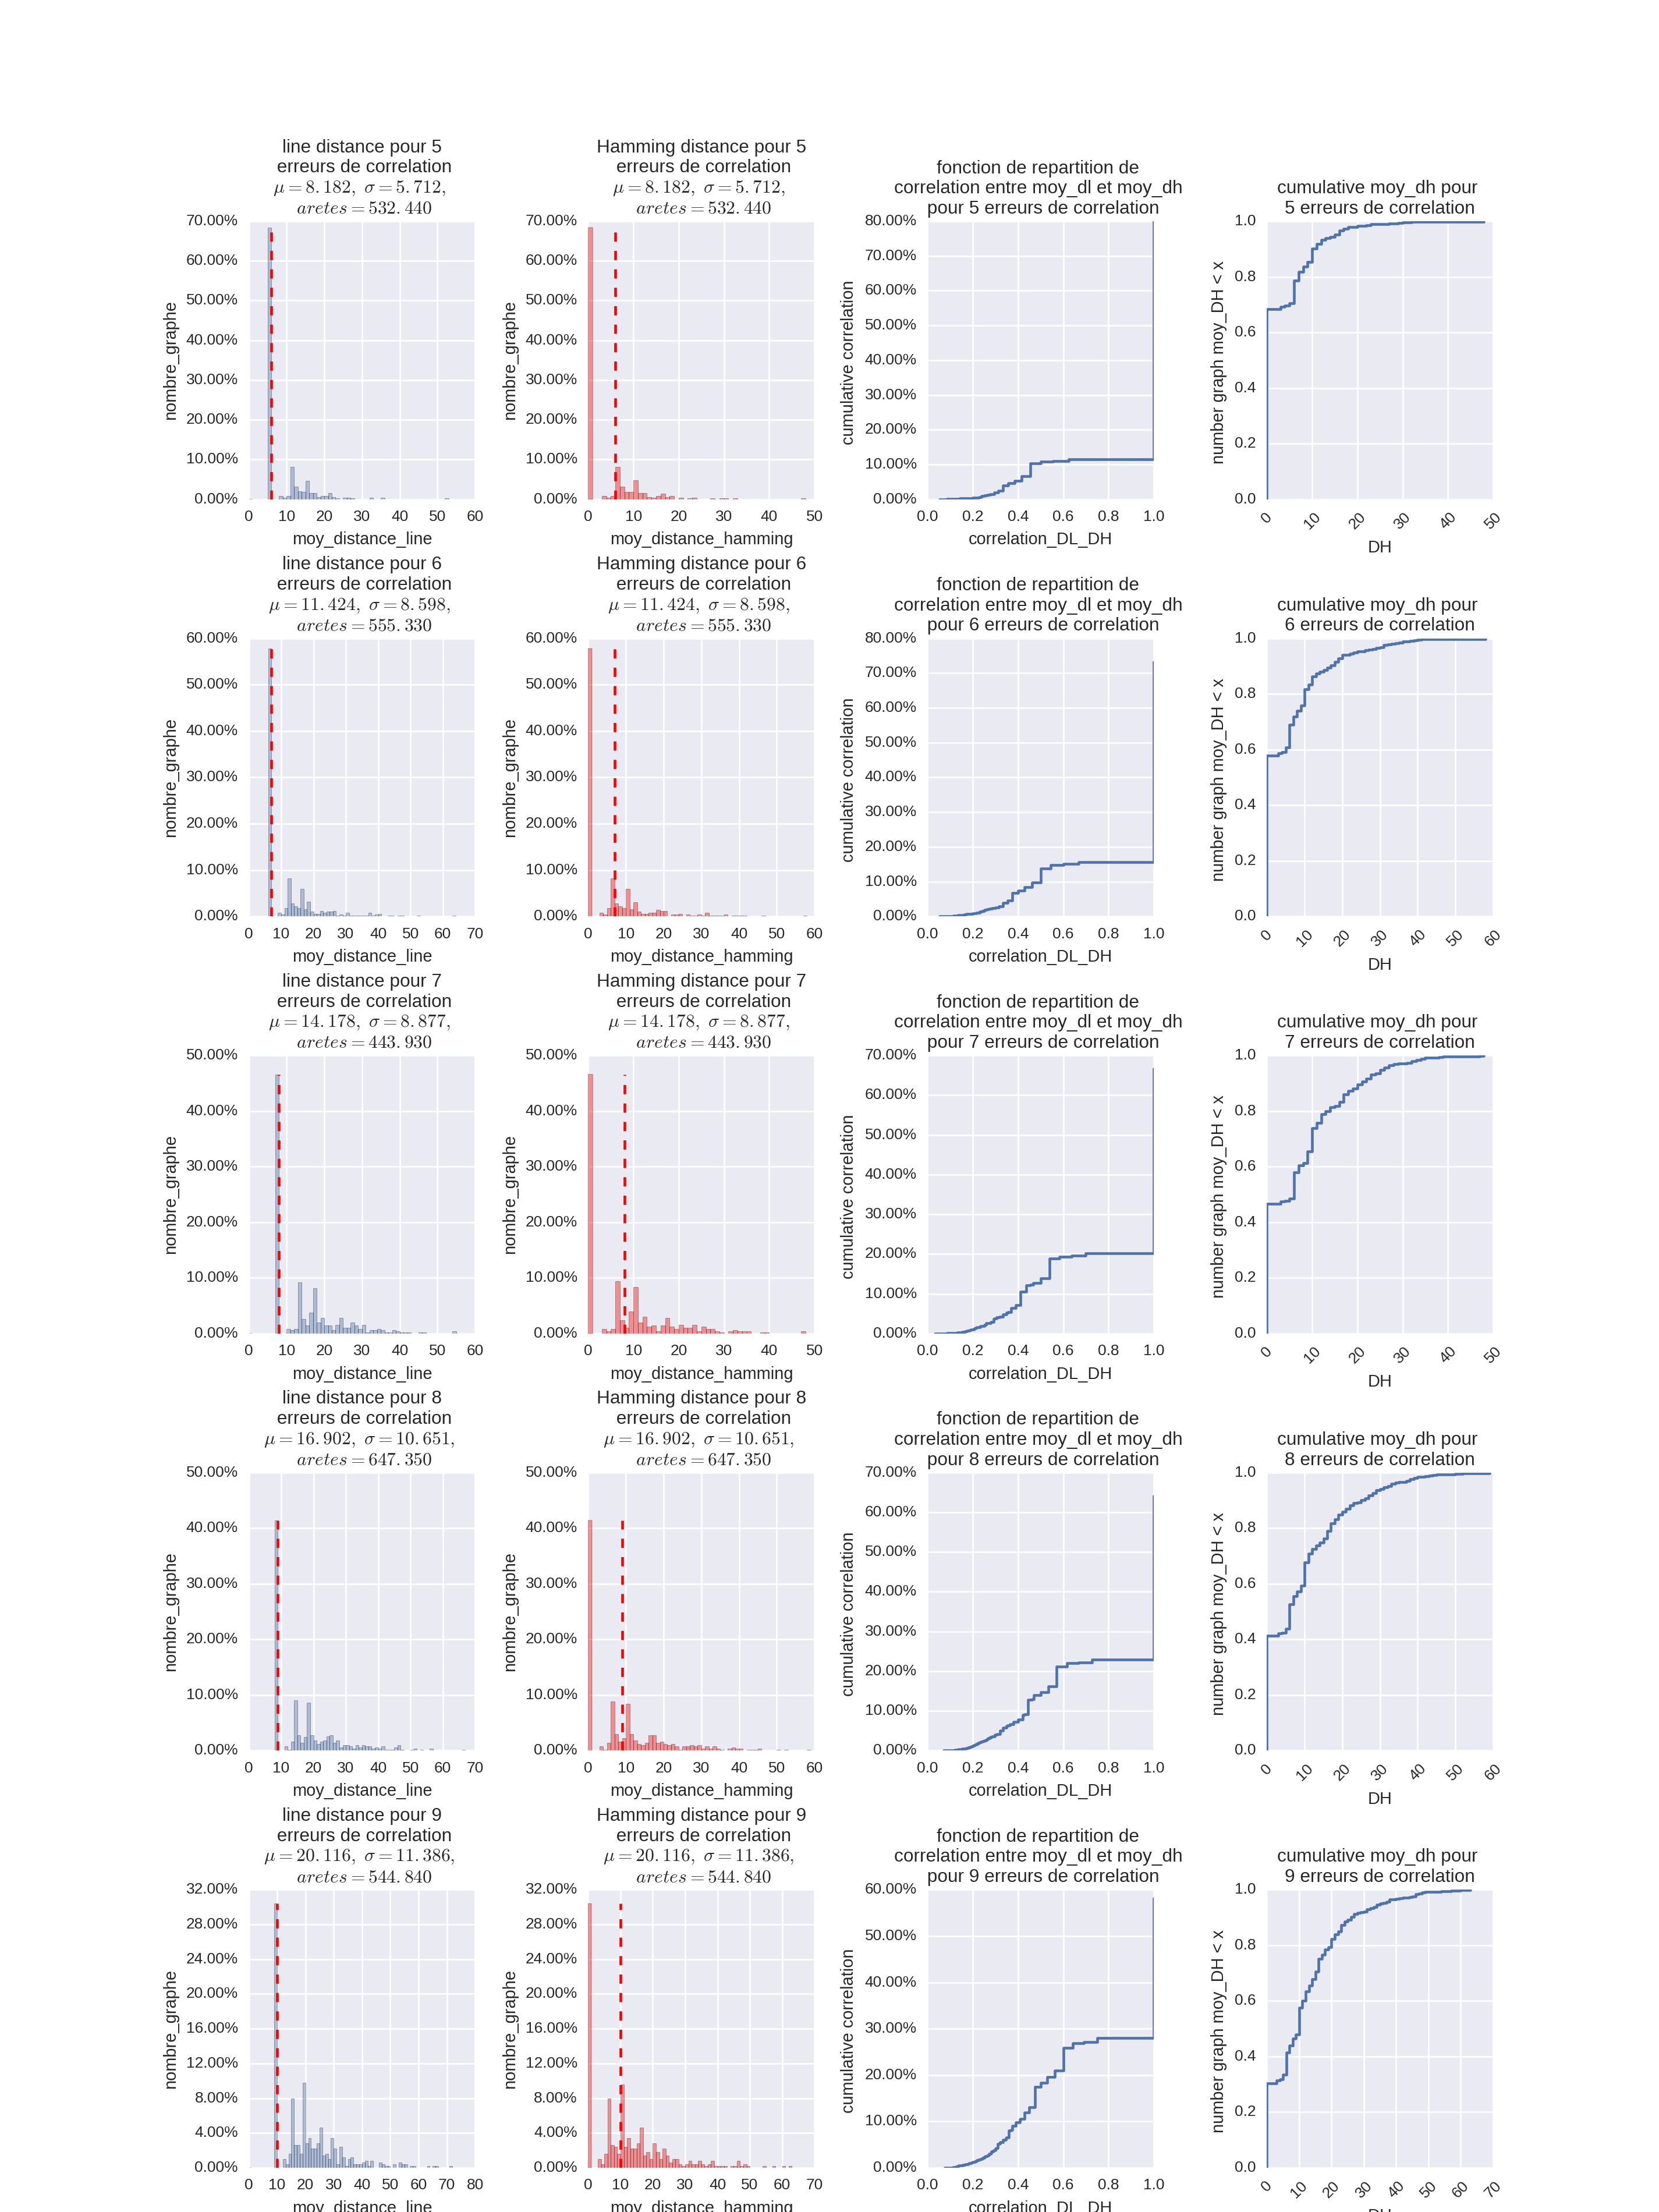
\includegraphics[width=550pt,height=600pt]{permut_distanceMoyenDLDH_k_5_9_aleatoire_p_10.jpeg}
\caption{ M\'ethode de permutation al\'eatoire avec une fonction de correction \`a co\^ut unitaire et $p\_correl = 1.0$ : distribution des distances line $moy\_DL$ et de Hamming $moy\_DH$ pour $k \in [6,  9]$ corr\'elations alter\'ees}
\label{permut_distanceMoyenDLDH_k_5_9_aleatoire_p_10} 
\end{figure}
%En revanche, ce pourcentage baisse malgr\'e le nombre \'elev\'e de corr\'elations {\em fausses positives}. Tel est le cas pour $k = 9$ corr\'elations o\`u le taux est de $24\%$. 
\newline
Par ailleurs, le mauvais r\'esultat obtenu pour des probabilit\'es $p\_correl < 0.5$ s'explique par le mode de fonctionnement de l'algorithme de correction. En Effet, cet algorithme consiste \`a ajouter des ar\^etes au voisinage du sommet \`a corriger puis \`a supprimer certaines ar\^etes pour \'eviter qu'un sommet n'appartienne \`a plus de $2$ cliques (propriet\'e du line graphe).
\newline
Nous pensons que le meilleur compromis est la probabilit\'e $p\_correl = 0.7$ parce que, pour peu de corr\'elations modifi\'ees ($k<5$), les lines-graphes produits $LG_k$ et g\'en\'er\'es $LG$ diff\`erent de $k<6$ ar\^etes correspondant aux $k$ erreurs de  corr\'elations effectu\'ees  et au d\'el\`a $k \geq 6$, le nombre d'ar\^etes diff\'erentes est fonction du nombre de corr\'elations faites multipl\'e par $1.5$.
Cela signifie qu'il faut, dans la matrice de corr\'elation, $30\%$ de corr\'elations {\em fausses positives} et $70\%$ de corr\'elation {\em fausses n\'egatives}. 
\newline
%Que se passe-t-il si on priorise l'ajout de corr\'elations {\em fausses n\'egatives} \`a chaque traitement c'est-\`a-dire la suppression d'ar\^etes?  
%En d'autres termes, l'ajout d'ar\^etes {\em fausses positives} a un co\^ut moins important que celui des {\em fausses n\'egatives}. 
%----
Que se passe-t-il si on priorise l'ajout de corr\'elations {\em fausses positives} \`a chaque traitement c'est-\`a-dire l'ajout d'ar\^etes?  
En d'autres termes, la suppression d'ar\^etes {\em fausses n\'egatives} a un co\^ut moins important que celui des {\em fausses positives}. 
%----
\subsubsection{Impact de la fonction de co\^ut sur les distributions}
\label{fonctionDeCout}

\begin{figure}[htb!] 
\centering
% a changer par des chemins relatifs
\includegraphics[scale=0.25]{simulation_comparaisonDifferentesFonctDeCout_by_aleatoire_p_correl_05.jpeg}
\caption{ Comparaison des diff\'erentes fonctions de co\^ut avec l'ajout de $k \in [1,9]$ de corr\'elations fausses positives et fausses n\'egatives pour une probabilit\'e $p = 0.5$ avec la m\'ethode de permutation al\'eatoire }
\label{compareDifferentesFonctionDeCout_p05} 
\end{figure}

Nous d\'efinissons quatre fonctions de co\^ut: unitaire (n=0), normal (n=1), quadratique (n=2), puissance 4 (n = 4) selon l'expression suivante
\begin{equation}
	\begin{aligned}
	F_n = 
	\begin{cases}
		prob[(a_i,a_j)]^n   \\
		(1 - prob[(a_i,a_j)])^n \\
	\end{cases}
	\end{aligned}
\end{equation}
ou $prob[(a_i,a_j)]^n$, la corr\'elation entre les ar\^etes $a_i$ et $a_j$, correspondant au co\^ut d'ajout de corr\'elations fausses n\'egatives, 
$(1-prob[(a_i,a_j)])^n$ au co\^ut d'ajout de corr\'elations fausses positives.
\newline
\'Etant donn\'ee que nous avons utilis\'e des matrices binaires dans la g\'en\'eration de line graphes, nous assignons des probabilit\'es pour chaque type de corr\'elation tel que:
\begin{itemize}
\item $prob[(a_i,a_j)] = [0, 0.5[ $ : corr\'elation vrai n\'egative i.e $0 \rightarrow 0$
\item $prob[(a_i,a_j)] = [0.5, 0.79[ $: corr\'elation fausse n\'egative i.e $1 \rightarrow 0$
\item $prob[(a_i,a_j)] = 0.8 $ : corr\'elation fausse positive i.e $0 \rightarrow 1$
\item $prob[(a_i,a_j)] = ]0.8, 1] $ : corr\'elation vrai positive i.e $1 \rightarrow 1$
\end{itemize}
La figure \ref{compareDifferentesFonctionDeCout_p05} affiche les courbes des diff\'erentes fonctions de co\^ut selon les $k$ corr\'elations modifi\'ees pour $p\_correl = 0.5$.
\newline
Les $4$ courbes sont superpos\'ees pour $k\le5$ et au d\'el\`a de $k>5$, les courbes carr\'ee (n=2) et normal (n=1) ont les plus petites distances moyenn\'ees de Hamming.
Pour $k>9$, la courbe unitaire (n=0) \'evolue de mani\`ere exponentielle tandis que les courbes quadratique (n=2) et normal (n=1) ont un rapport de $2$ entre les distances de Hamming et le nombre $k$ de corr\'elations modifi\'ees.
On en d\'eduit que la pire fonction de co\^ut est la fonction unitaire (n=0 en jaune).
\newline
Cependant, nous ne pouvons pas choisir la meilleure fonction de co\^ut car les fonctions des courbes {\em normal} et {\em quadratique} \'evoluent identiquement.
 On peut conclure qu'utiliser les probabilit\'es de corr\'elations pour le calcul du co\^ut am\'eliore significativement les distances moyenn\'ees de Hamming.
 \newline
 On choisit pour la suite la fonction de co\^ut normal $F_1$ pour le co\^ut de modification de chaque ar\^ete. 

\paragraph{Cas particulier: fonction de co\^ut en cloche}

%petit rappel sur comment fonctionne la correction avec les autres fonctions de cout
Souvenons nous que corriger la matrice binaire de corr\'elation consiste \`a modifier les cases de cette matrice par leurs valeurs contraires.
Le cas id\'eal serait la modification des corr\'elations fausses positives et fausses n\'egatives pendant la phase de correction.
Cependant, pendant cette phase, la correction est effectu\'ee autant sur les corr\'elations fausses positives et fausses n\'egatives que sur celles vrai positives et vrai n\'egatives.
L'algorithme de correction ne fait aucune distintion entre les corr\'elations fausses et les bonnes corr\'elations.
Afin de prioriser la modification des corr\'elations fausses, nous definisons une nouvelle fonction de co\^ut appel\'ee {\em cloche}.
\newline
% definir la fonction de cloche et sa particularite
La fonction {\em cloche} se d\'efinit ainsi:
\begin{equation}
	F_c = | 4\cdot((p-s) - (s-0.5))^2 |^{1.5}  
\end{equation}
La fonction de co\^ut cloche est une fonction polynomiale de degr\'e $2$ qui applique des poids aux ar\^etes de sorte que les ar\^etes, dont les corr\'elations tendent vers le seuil, sont moins p\'enalis\'ees et les ar\^etes, dont les corr\'elations sont \'eloign\'ees du seuil, ne sont quasi jamais utilis\'ees pendant la phase de correction. 
Les poids minimaux sont appliqu\'es pour les corr\'elations fausses tandis que les poids maximaux (= $1$) sont appliqu\'es aux bonnes corr\'elations
%La fonction de co\^ut cloche est une fonction polynomiale de degr\'e $2$ qui applique les co\^uts les plus \'elev\'es aux corr\'elations exactes (c'est-\`a-dire $1$) et les co\^uts les plus faibles aux corr\'elations fausses.
Cette fonction depend de la valeur de corr\'elation $p$ entre deux ar\^etes et du seuil $s$ \`a partir duquel on introduit des corr\'elations erron\'ees.
\newline
% comparaison entre les fonctions de cout unitaire, lineaire et en cloche

Les algorithmes (couverture et correction) sont ex\'ecut\'ees avec la fonction cloche sur les graphes g\'en\'er\'es pr\'ec\'edemment. 
Les diff\'erentes distances line/Hamming obtenues, compar\'ees avec les fonctions de co\^uts unitaires $F_0$ et normales $F_1$, sont r\'esum\'ees dans la figure \ref{comparaison_fct_cloche_unitaire_normal_p05}.
En effet, pour $10$ et $20$ erreurs de corr\'elation, l'algorithme de correction modifie  de $11$ \`a $22$ ar\^etes pour la fonction normale $F_1$ et aussi de $38$ \`a $65$ pour la fonction en cloche respectivement. 
% expliquer
Nous en deduisons que le co\^ut de la fonction $F_1$ est  inf\'erieur \`a celui de la fonction en cloche. 
La figure \ref{comparaison_fct_cloche_unitaire_normal_p05}  est une bonne illustration par la position de la courbe rouge ($F_1$) en dessous de celle en jaune ($cloche$).
\newline
Ce resultat provient de l'utilisation des ar\^etes fausses n\'egatives parce que le co\^ut de ces ar\^etes est faible par rapport au co\^ut des ar\^etes de corr\'elations fausses positives.
En effet les corr\'elations fausses n\'egatives et fausses positives appartiennent aux intervalles $[0,s[$ et $]s,1]$ respectivement. 
Alors qu'on a une d\'ecroissance faible de $0$ \`a $s$ et une croissance forte de $s$ \`a $1$ dans la courbe de $F_c$. 
Ce qui explique le co\^ut faible des fausses n\'egatives et celui \'elev\'e des fausses positives. 
Par ailleurs, la courbe en bleu (fonction unitaire $F_0$) est au dessus des deux autres courbes ($F_1$ et cloche) indiquant que son co\^ut est le plus \'elev\'e des trois fonctions.
\newline
%% ---- REPROGRAMMER
\begin{figure}[htb!] 
\centering
% a changer par des chemins relatifs
\includegraphics[scale=0.25]{simulation_comparaisonDifferentesFonctDeCout_by_aleatoire_p_05.jpeg}
\caption{ Comparaison des fonctions de co\^ut unitaire, normal et en cloche avec l'ajout de $k \in [1,9]$ de corr\'elations fausses positives et fausses n\'egatives pour une probabilit\'e $p = 0.5$ avec la m\'ethode de permutation al\'eatoire }
\label{comparaison_fct_cloche_unitaire_normal_p05} 
\end{figure}
%% ---- REPROGRAMMER
%Conclusion
On en conclut, par transitivit\'e, que la fonction $F_1$ fournit les co\^uts minimum pendant la correction.

% section de definition de parametres pour avoir le line graphe de distance de Hamming minimale.



%#############################
%#               correction graphes iourtes           #
%#############################
\section{Correction des Graphes Iourtes}


%#############################
%#               conclusion				          #
%#############################
\section{Conclusion}

\end{document}